\documentclass[lang=en]{elegantpaper}   

\title{Liver E13.5 Clustering Report}
\author{Xun Zhao}
\date{\today}

\begin{document}
\maketitle

\section{Seurat Codes and Parameters}
% Codes here
\section{Clustering and Annotation}

\subsection{Clustering}

\begin{figure}[htbp]
    \centering
    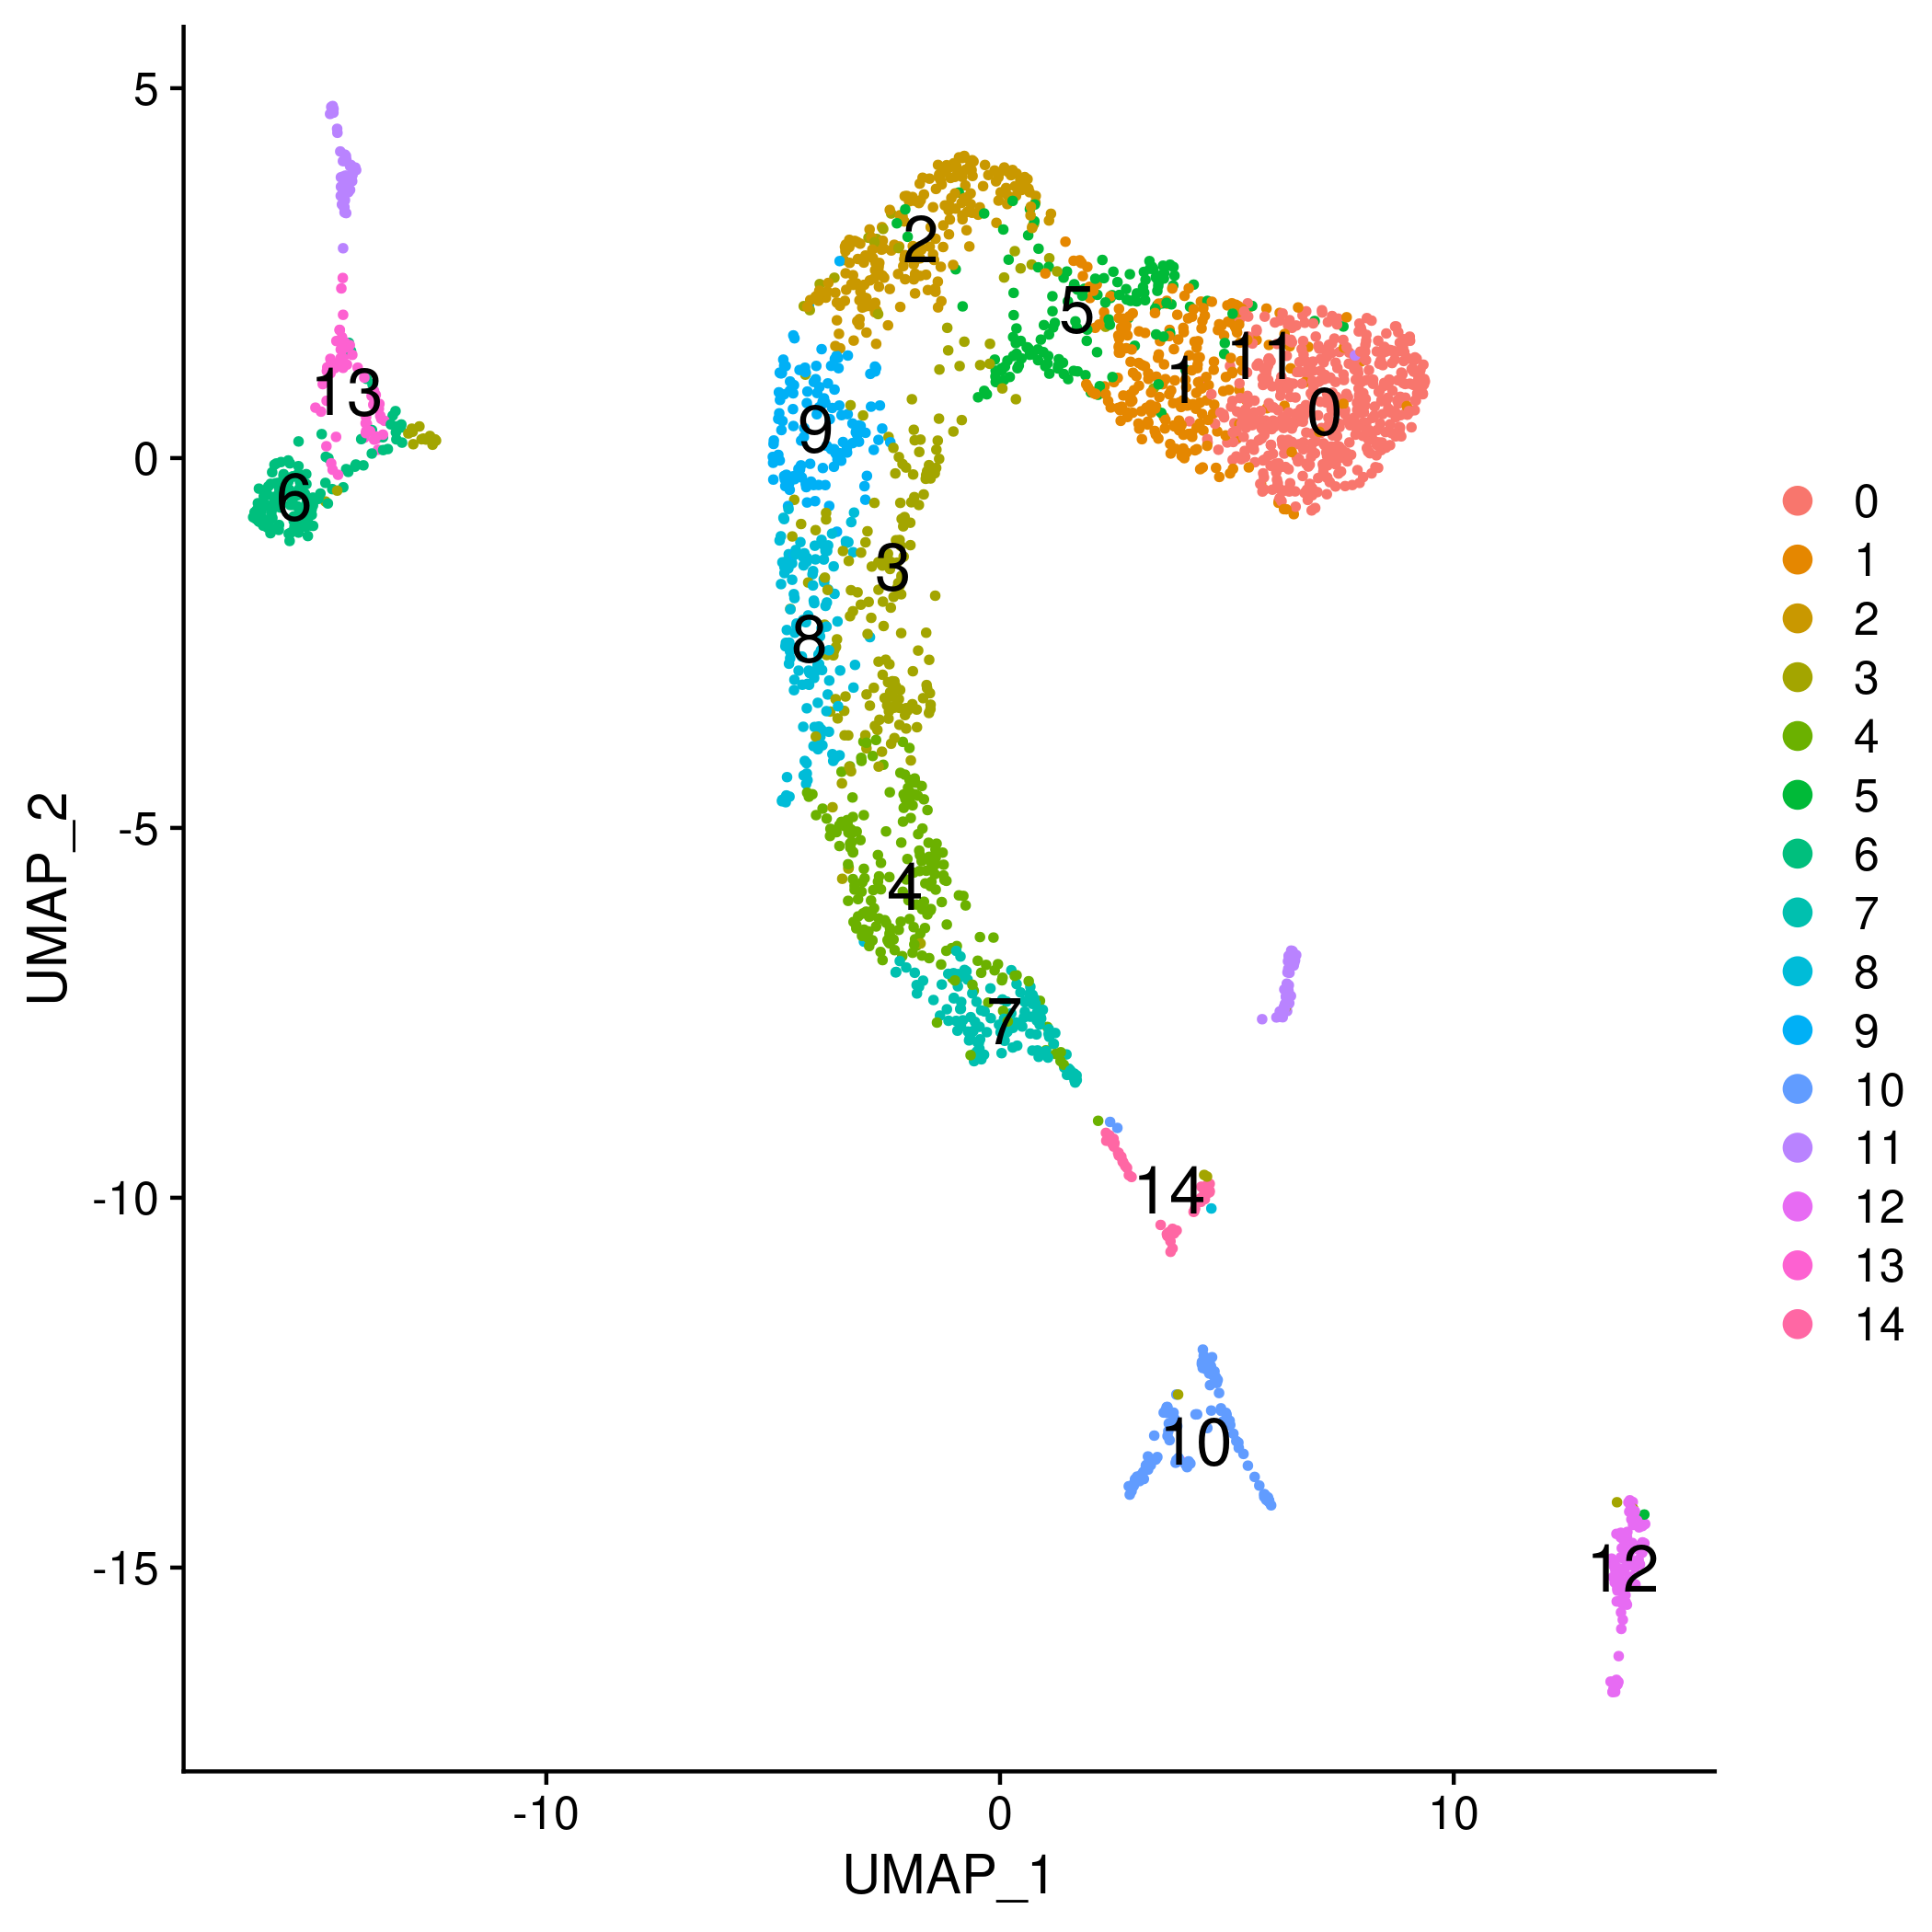
\includegraphics[width=0.6\textwidth]{image/d.png}
    \caption{Unlabeled Clusters \label{d}}
\end{figure}

\figref{d} is clustering result using 0.8 resolution. RDS file is available in \lstinline{/p200/liujiang_group/yinyao/Dataset/Seurat/Liver.rds}. After extracting markers, some of these clusters can be annotated, but others need further clustering, like C11 (cluster 11, purple), which consists of two parts away form each other.

\subsection{Annotation}

\emph{Afp}, \emph{Alb} are reported as the markers of hepatocyte or hepatoblast\citep{gordillo_orchestrating_2015, chaudhari_expression_2016, su_single-cell_2017, han_mapping_2018}. Moreover, besides \emph{Afp} and \emph{Alb}, hepatocyte also expresses \emph{Hnf4$\alpha$} and \emph{Prox1}\citep{gordillo_orchestrating_2015}. Therefore, C6 and C13 are annotated as hepatocyte and hepatoblast, respectively, for their high expression of \emph{Afp} and \emph{Alb}, and for expression of \emph{Hnf4$\alpha$} and \emph{Prox1} in C13 (\figref{f613}).

\begin{figure}[htbp]
    \centering
    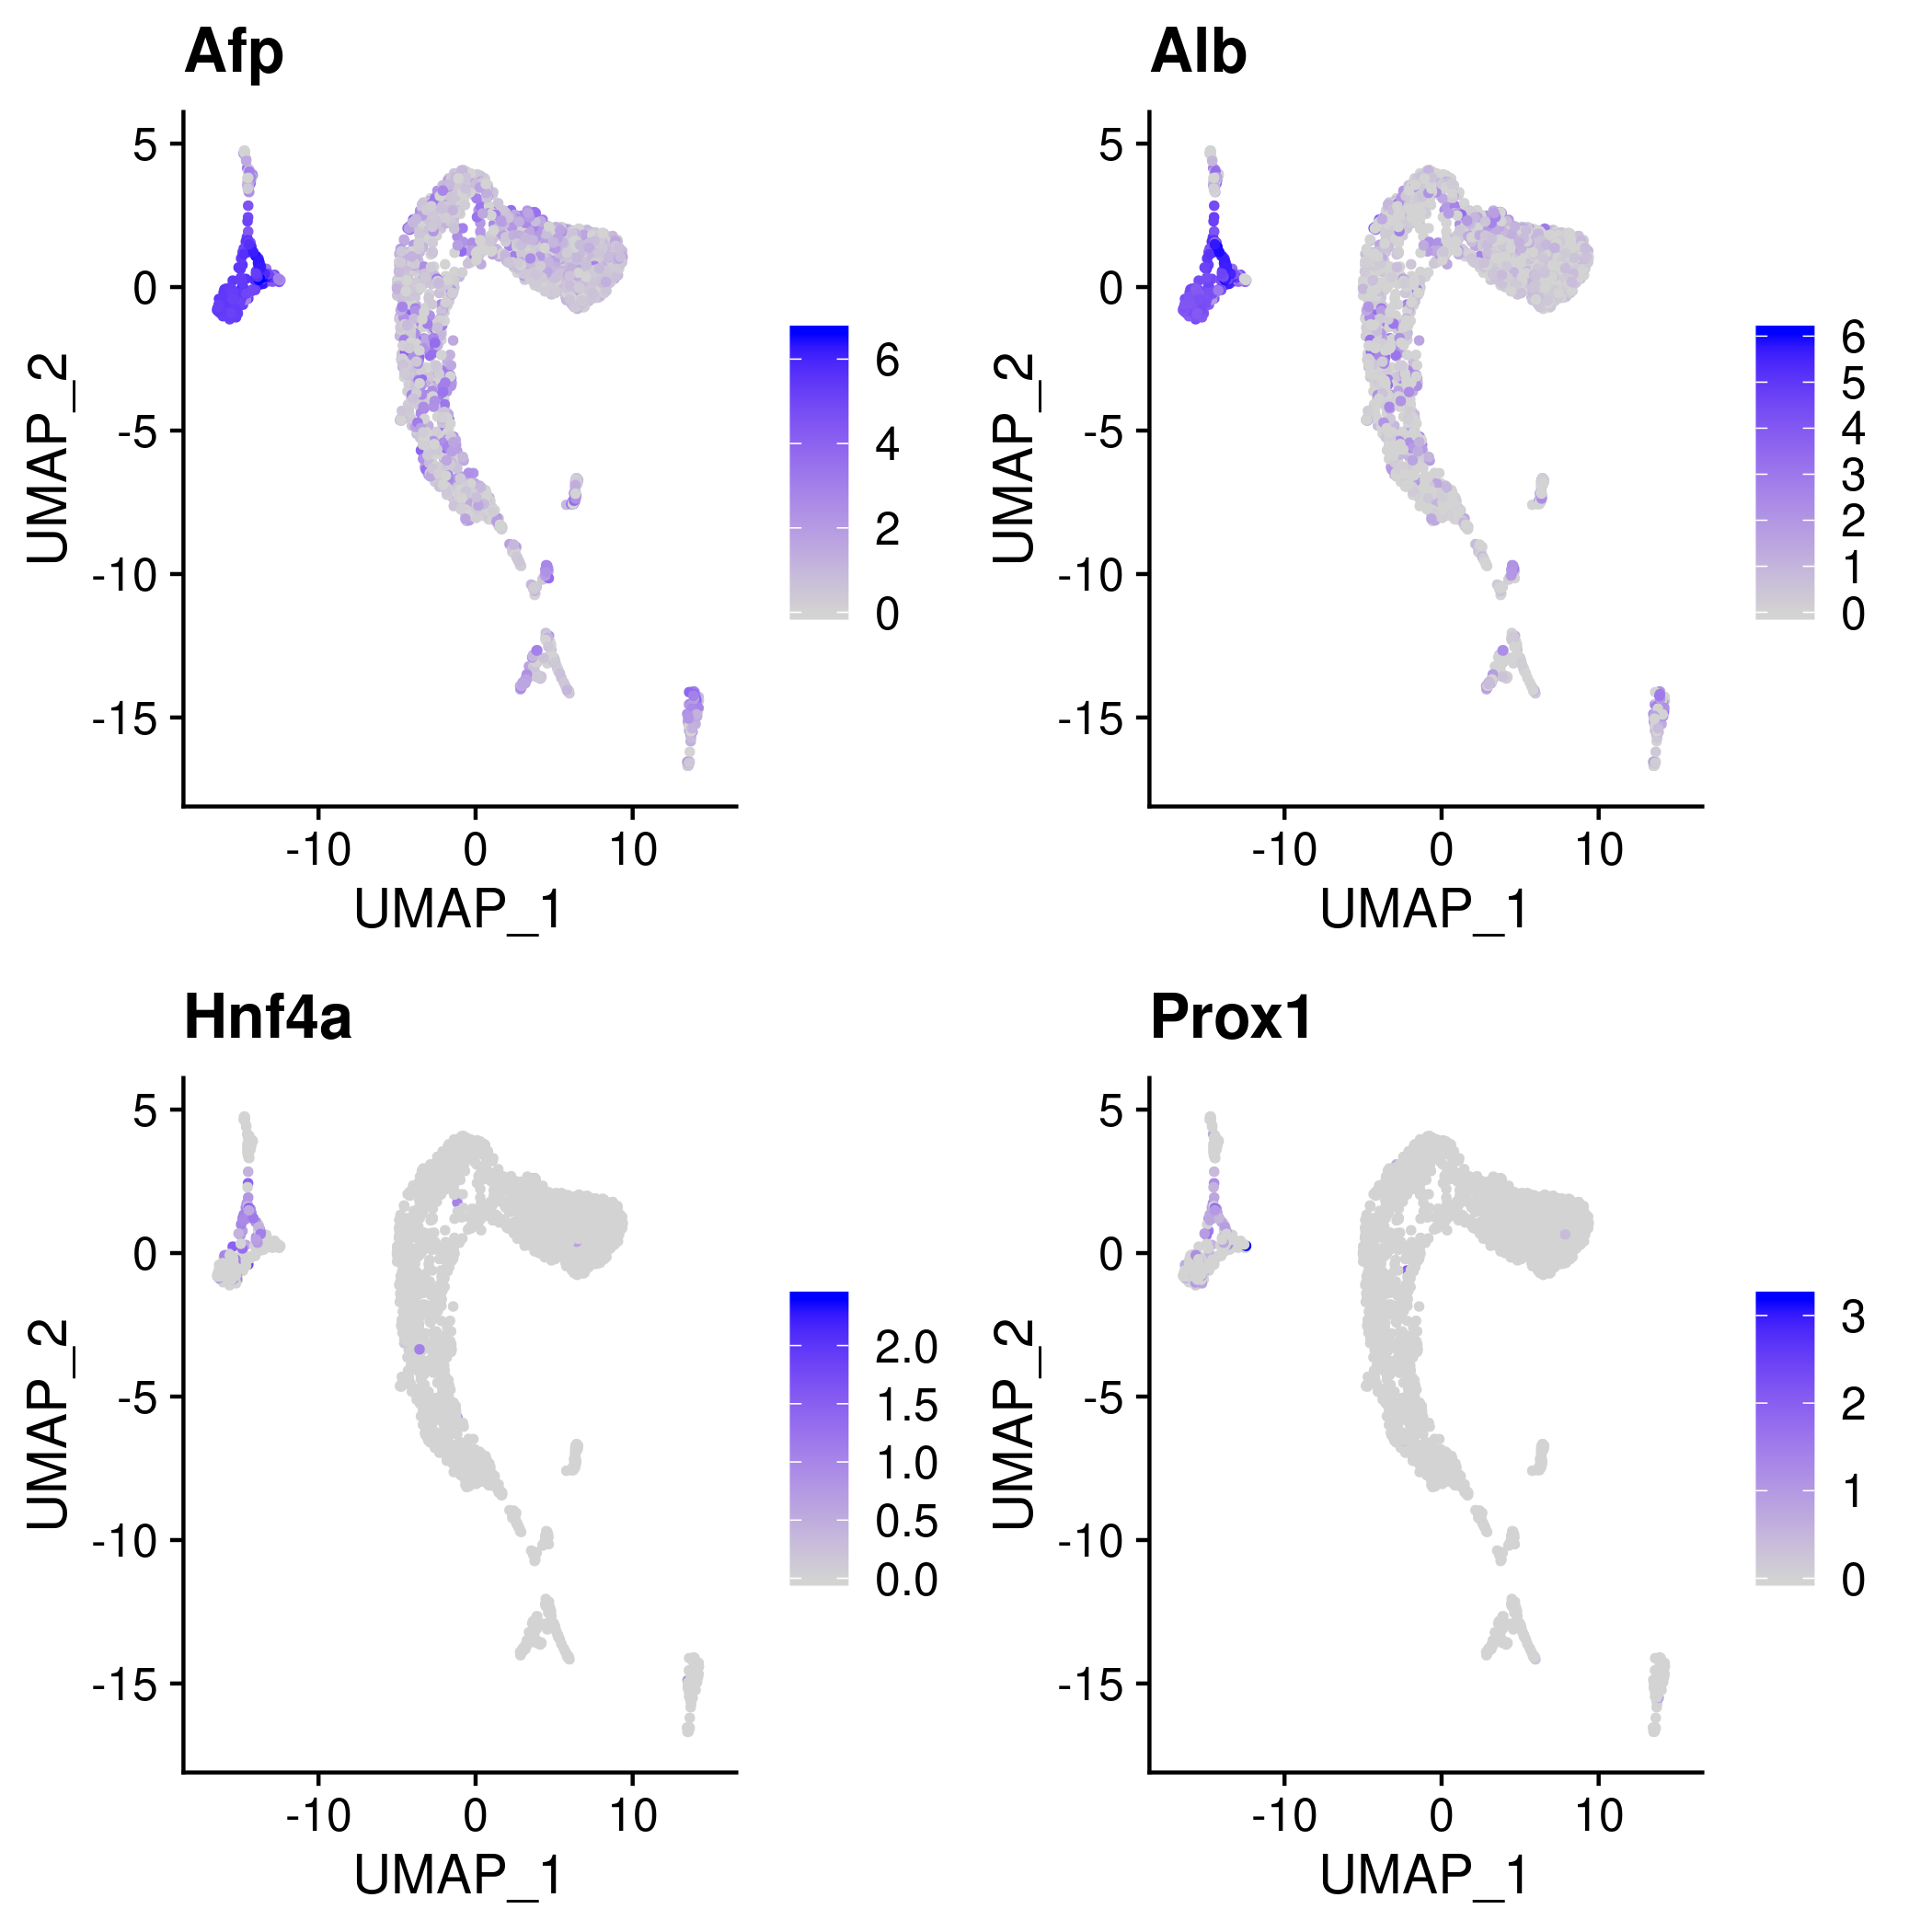
\includegraphics[width=0.6\textwidth]{f613.png}
    \caption{Markers of C6/C13 \label{f613}}
\end{figure}

\emph{Cd68, Marco} are reported as the markers of macrophage\citep{su_single-cell_2017, han_mapping_2018}, so C12 is annotated as macrophage. \emph{Ppbp, Itga2b} are reported as the markers of megakaryocyte\citep{su_single-cell_2017}, so C14 is annotated as megakaryocyte (\figref{f1214}).

\begin{figure}[htbp]
    \centering
    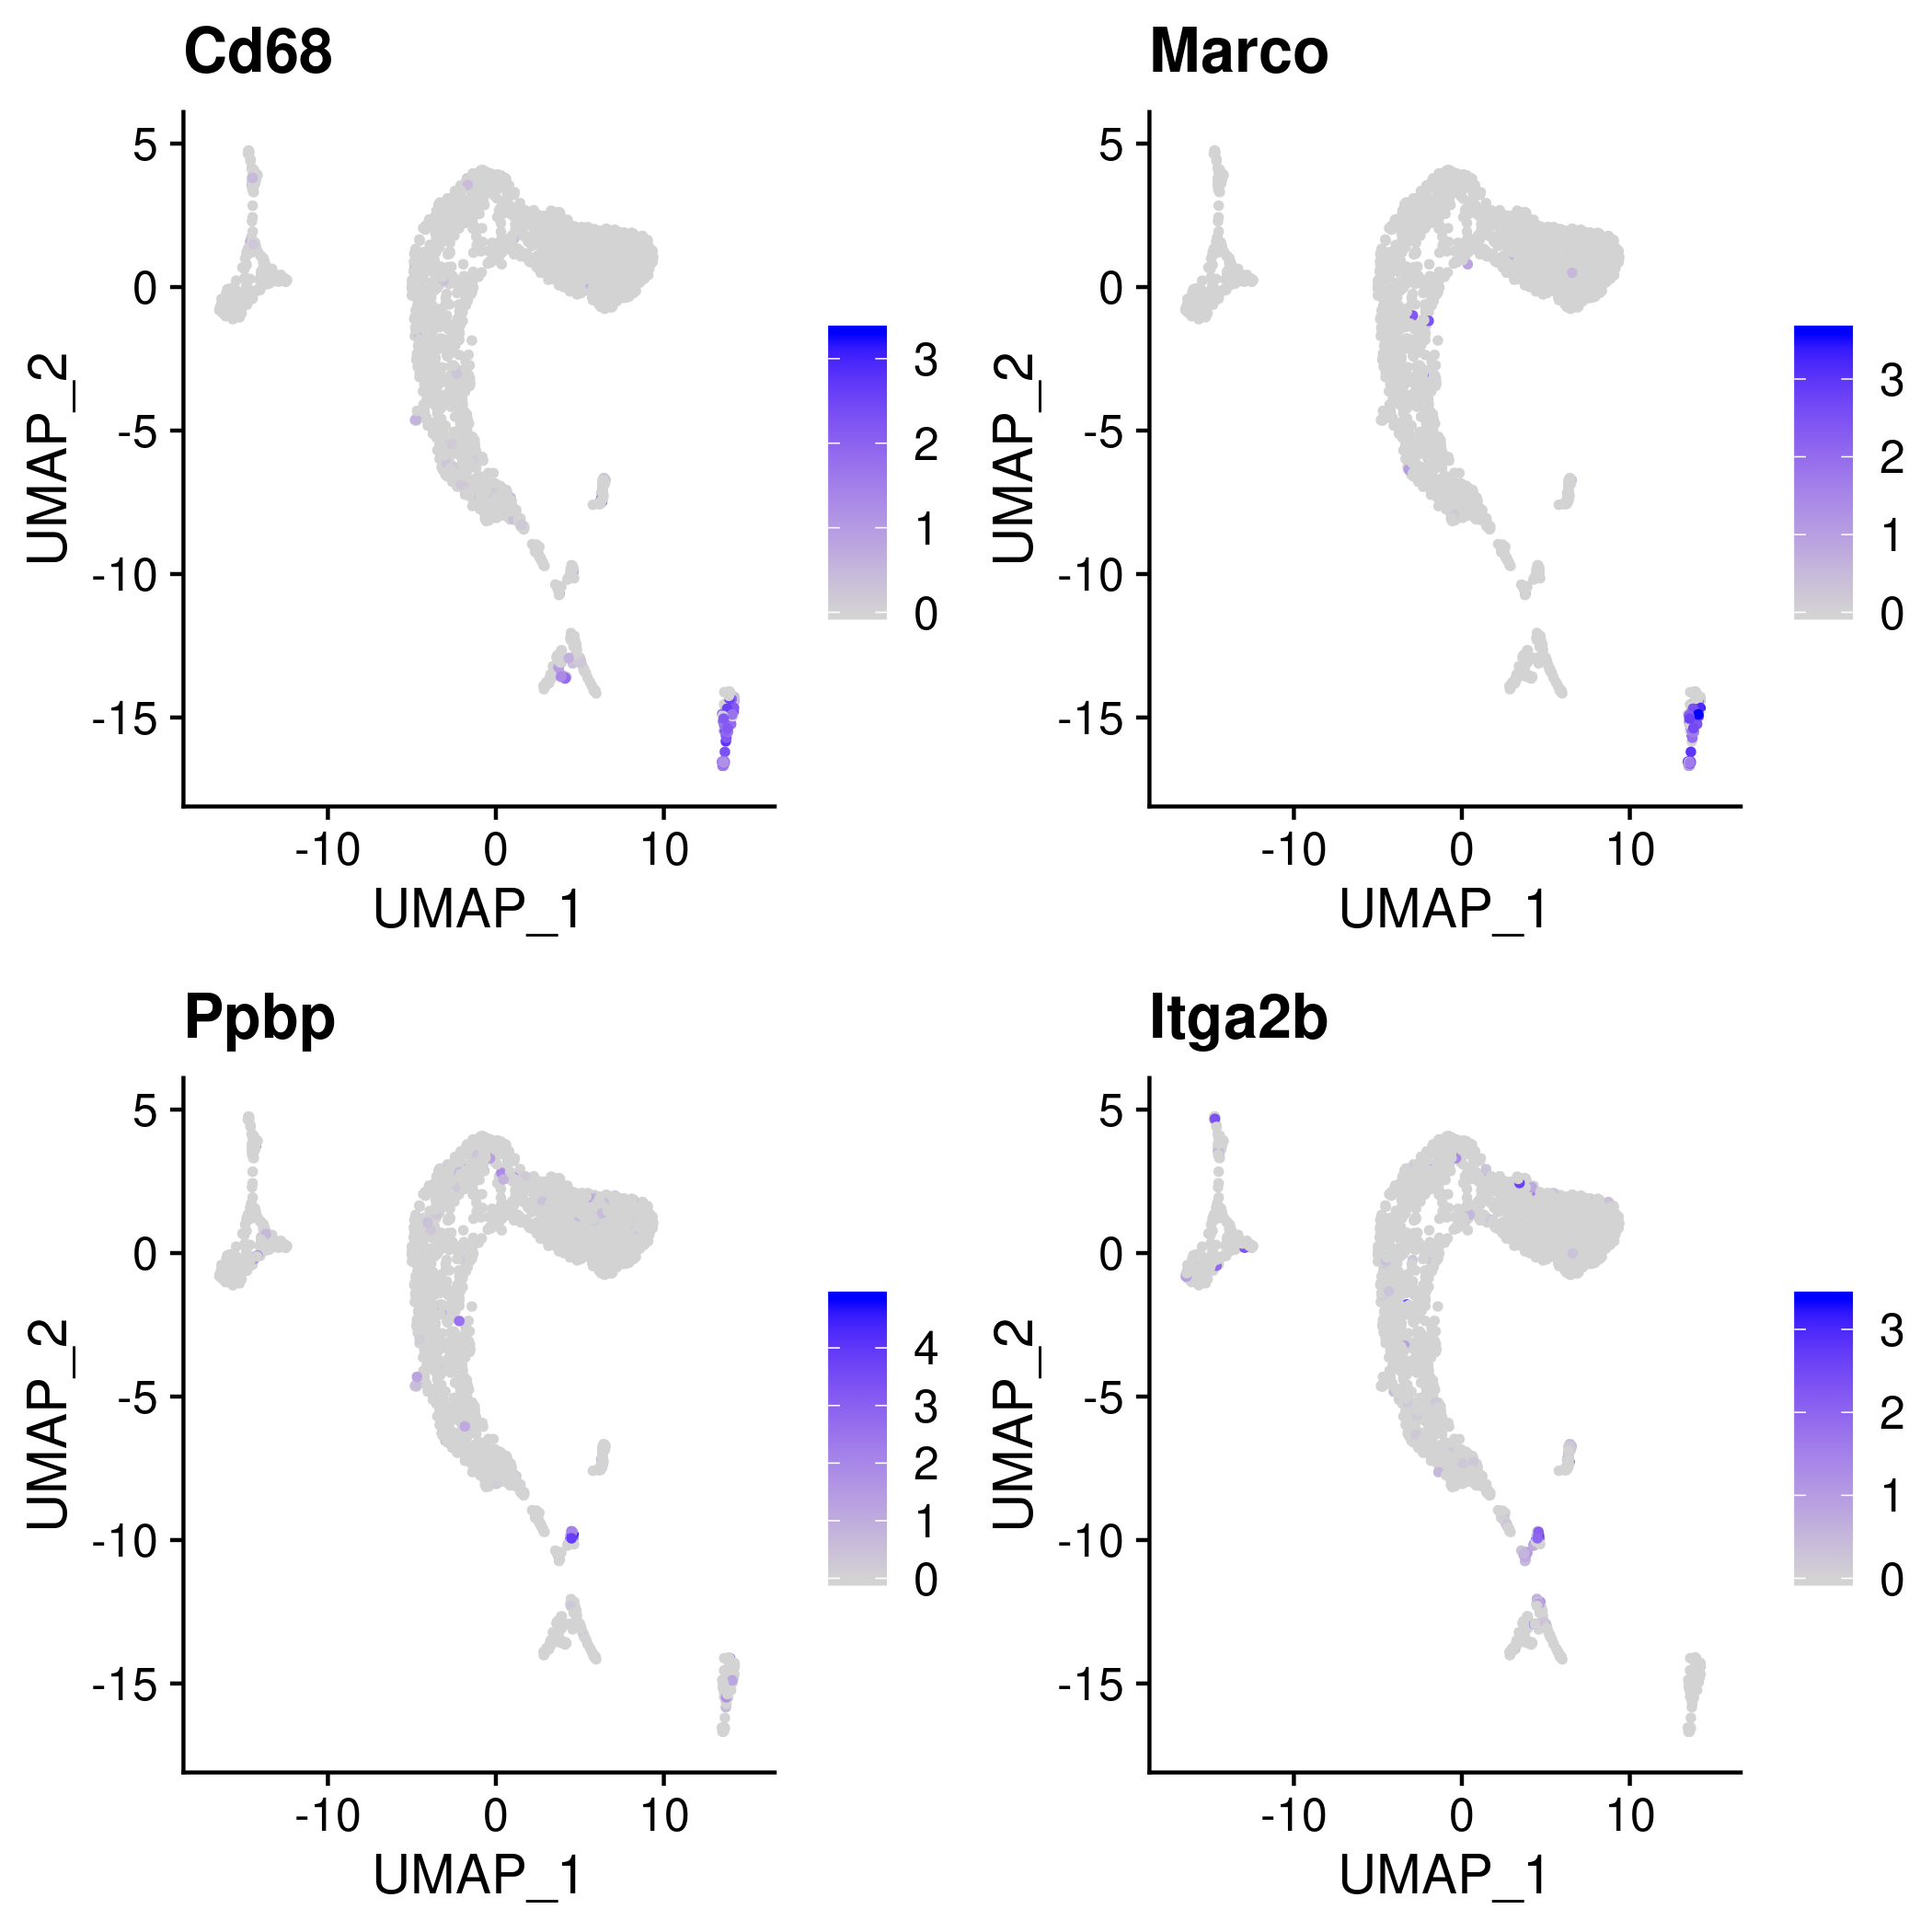
\includegraphics[width=0.6\textwidth]{f1214.png}
    \caption{Markers of C12/C14 \label{f1214}}
\end{figure}

In the main body of \figref{d} (C0-5, C7-9), \emph{Hba-a2, Hba-a1, Hbb-bs, Hbb-bt}, the markers of erythroid\citep{han_mapping_2018}, express higher in C0, C1, C5 (\figref{fe}). \emph{Klf1, Alad, Blvrb, Gata1}, the markers of erythroid progenitor\citep{han_mapping_2018}, express higher in C2, C7, C8, C9 (\figref{fep}). Both erythroid and erythroid progenitor markers are not significant in C3, so C3 is not annotated yet.

\begin{figure}[htbp]
    \centering
    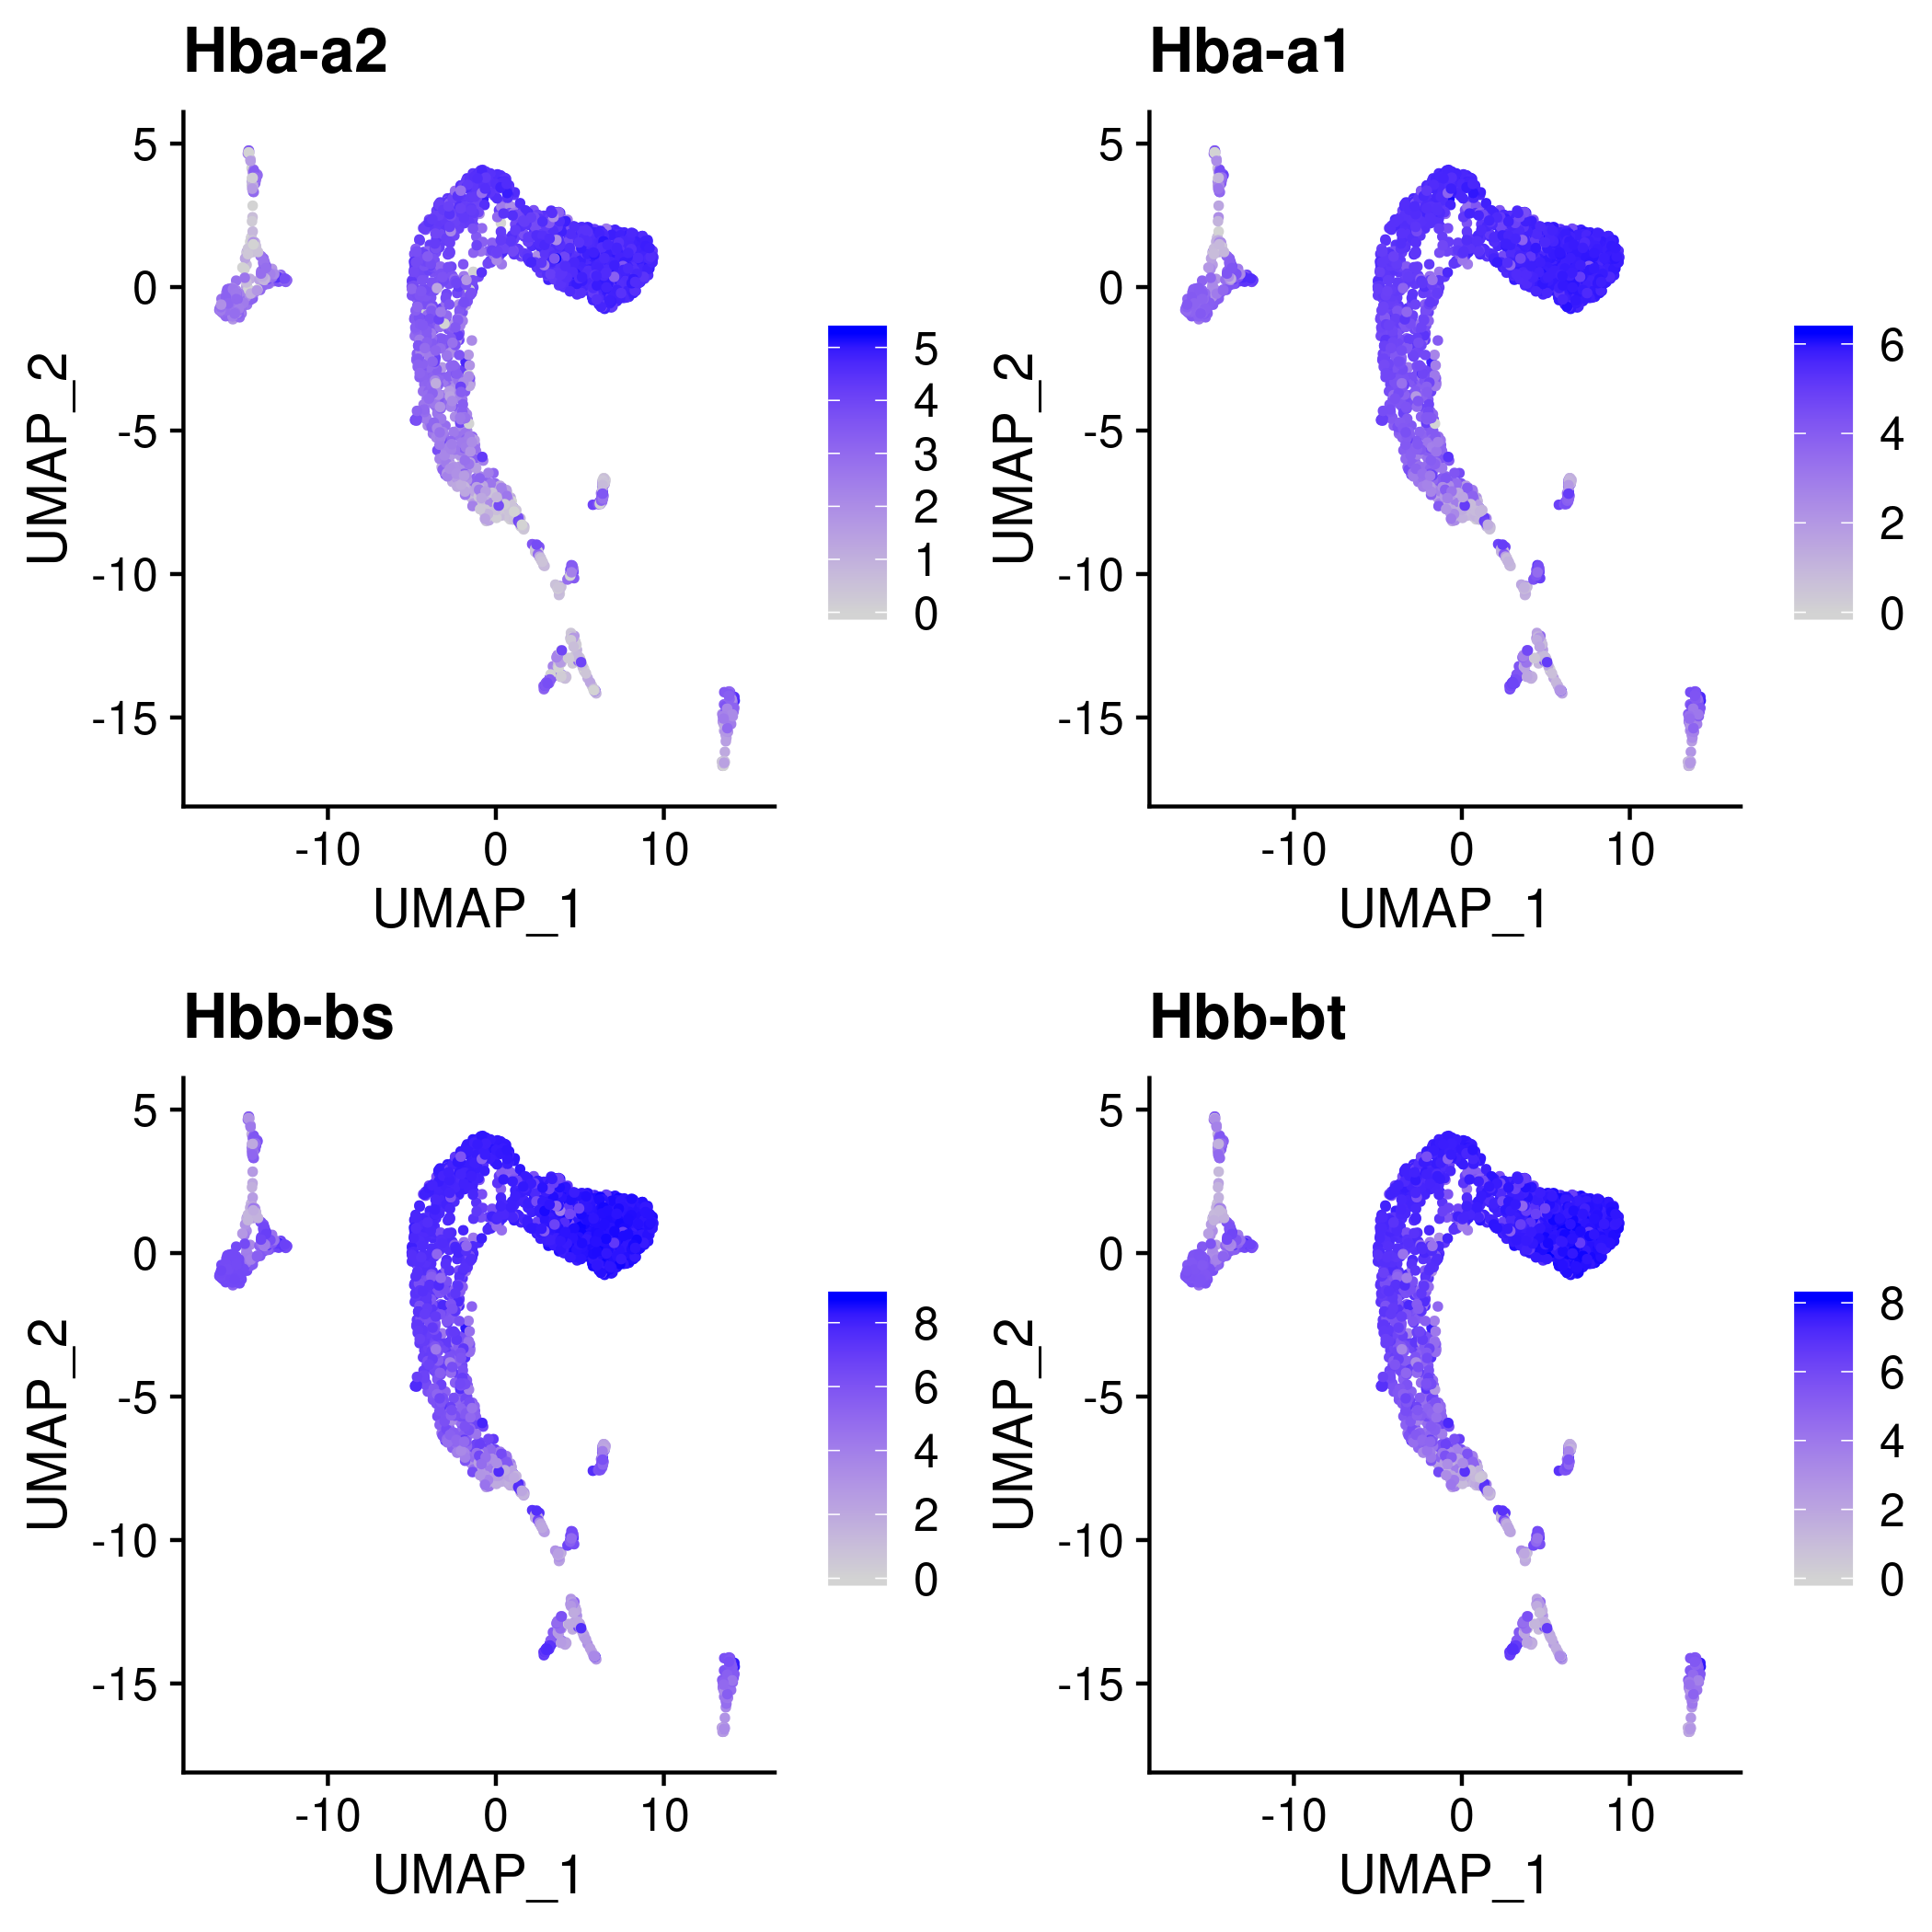
\includegraphics[width=0.6\textwidth]{image/fe.png}
    \caption{Markers of Erythroid \label{fe}}
\end{figure}
\begin{figure}[htbp]
    \centering
    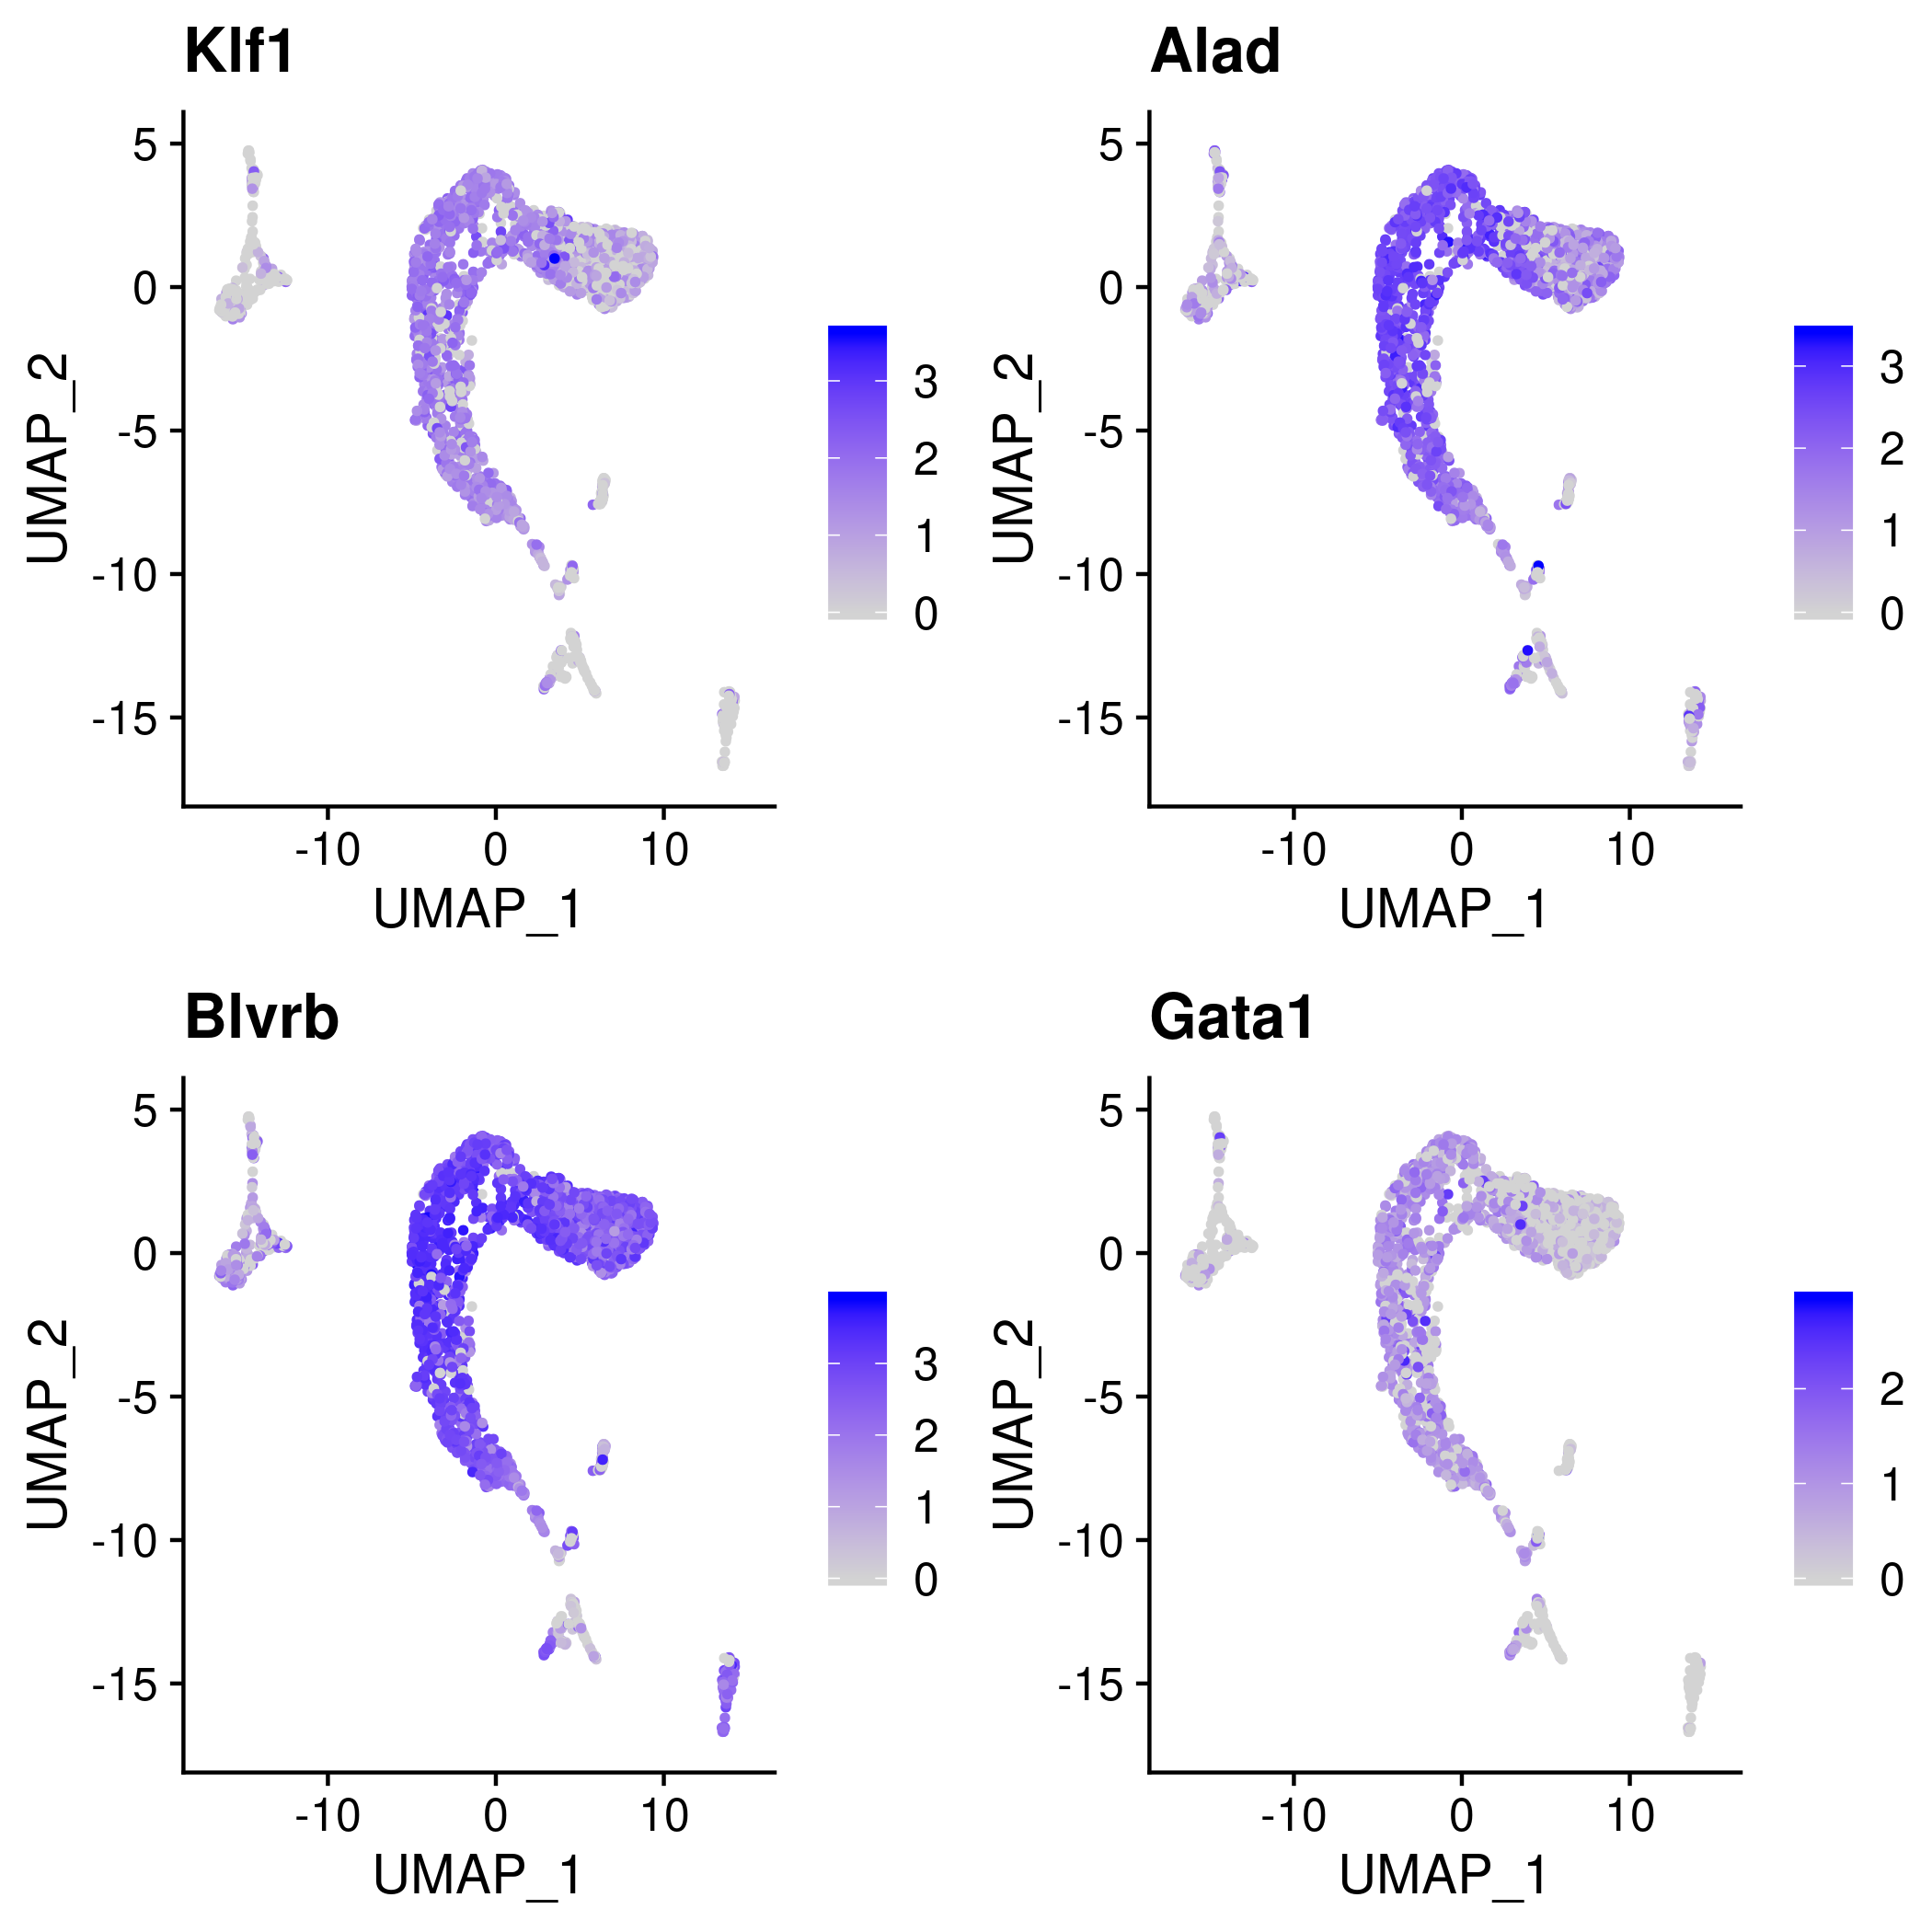
\includegraphics[width=0.6\textwidth]{image/fep.png}
    \caption{Markers of Erythroid Progenitor\label{fep}}
\end{figure}

However, in C10, there are two kinds of cell markers, stem cells' and neutrophils'. Similarly, in C11, there are endothelial cells' and mesenchymal cells'. So they need further clustering.

\subsection{Subclustering}

In order to simply divide one cluster into fewer parts, the resolution used in this part is 0.6. 

\paragraph{Cluster 10} C10 is divided into 3 parts (\figref{d10}), saved as \lstinline{/p200/liujiang_group/yinyao/Dataset/Seurat/liver10.rds}. Stem cell marker \emph{Cd34, Cmtm7}\citep{han_mapping_2018} are highly expressed in subcluster 0 of C10. Neutrophil marker \emph{S100a9, S100a8}\citep{han_mapping_2018} are highly expressed in subcluster 2 of C10 (\figref{f10}, \figref{f10t}). The annotation of subcluster 1 is not defined yet.

\begin{figure}[htbp]
    \centering
    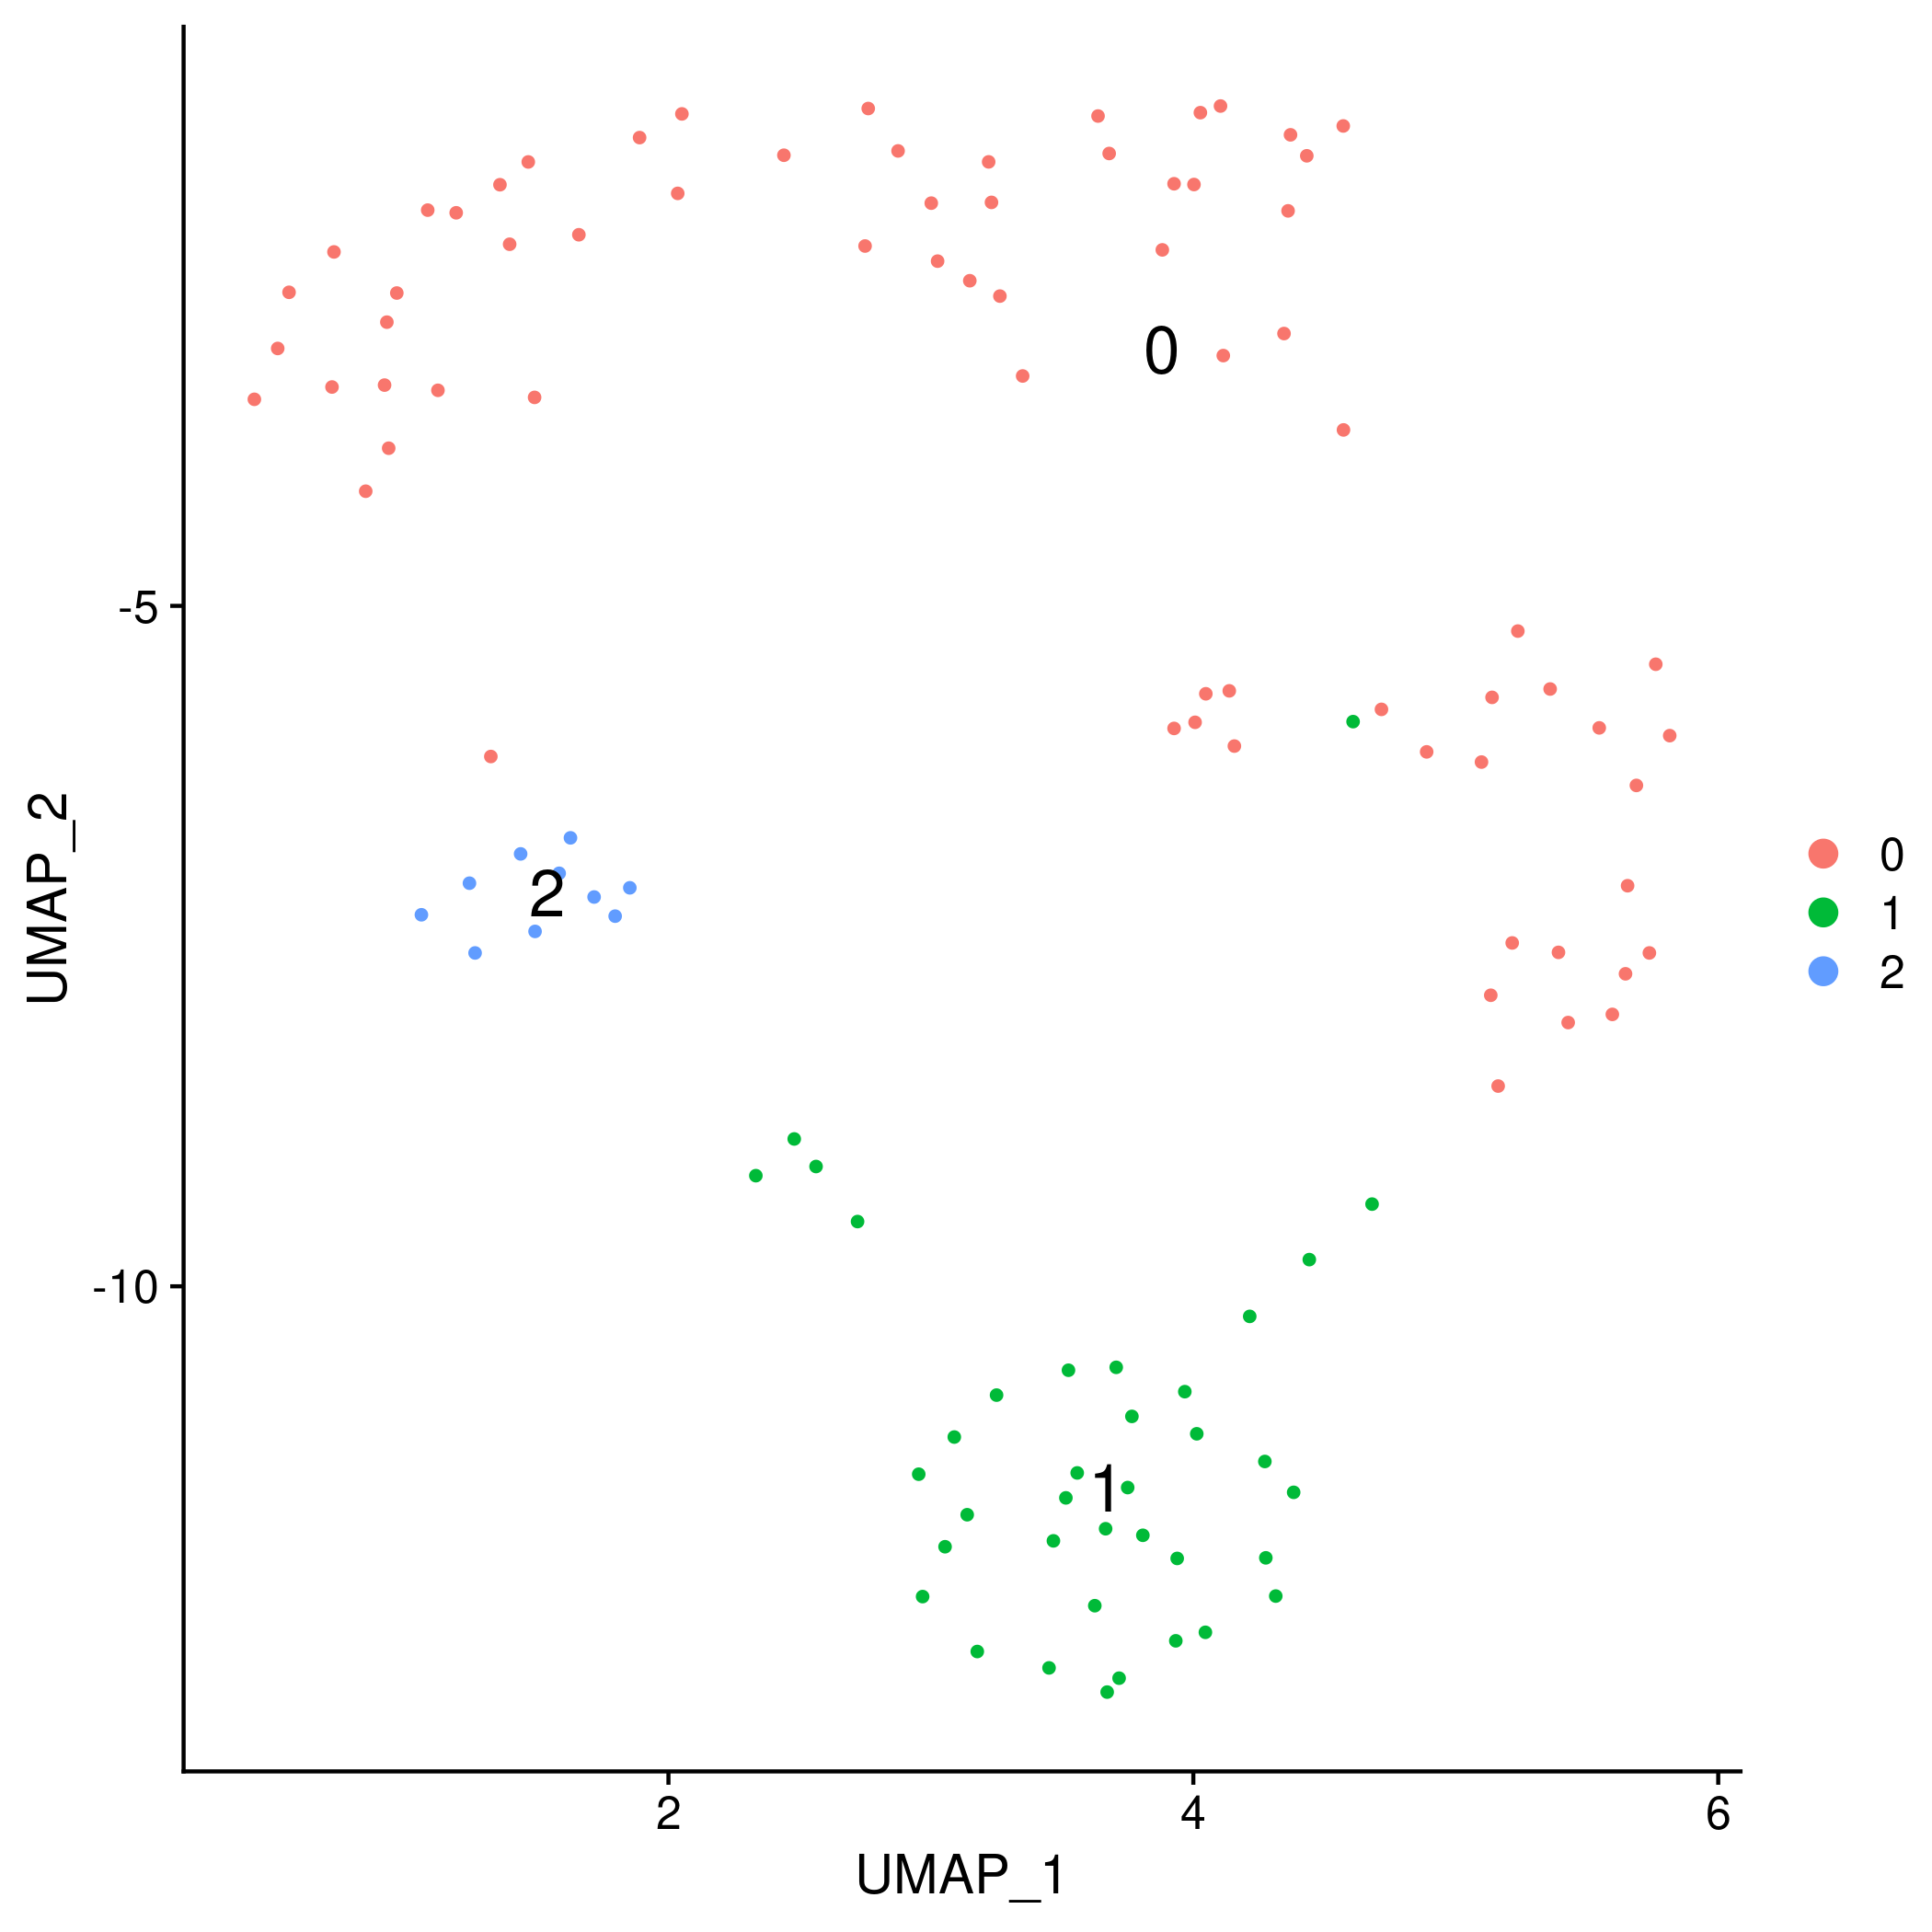
\includegraphics[width=0.6\linewidth]{image/d10.png}
    \caption{Subclusters of C10 \label{d10}}
\end{figure}
\begin{figure}[htbp]
    \centering
    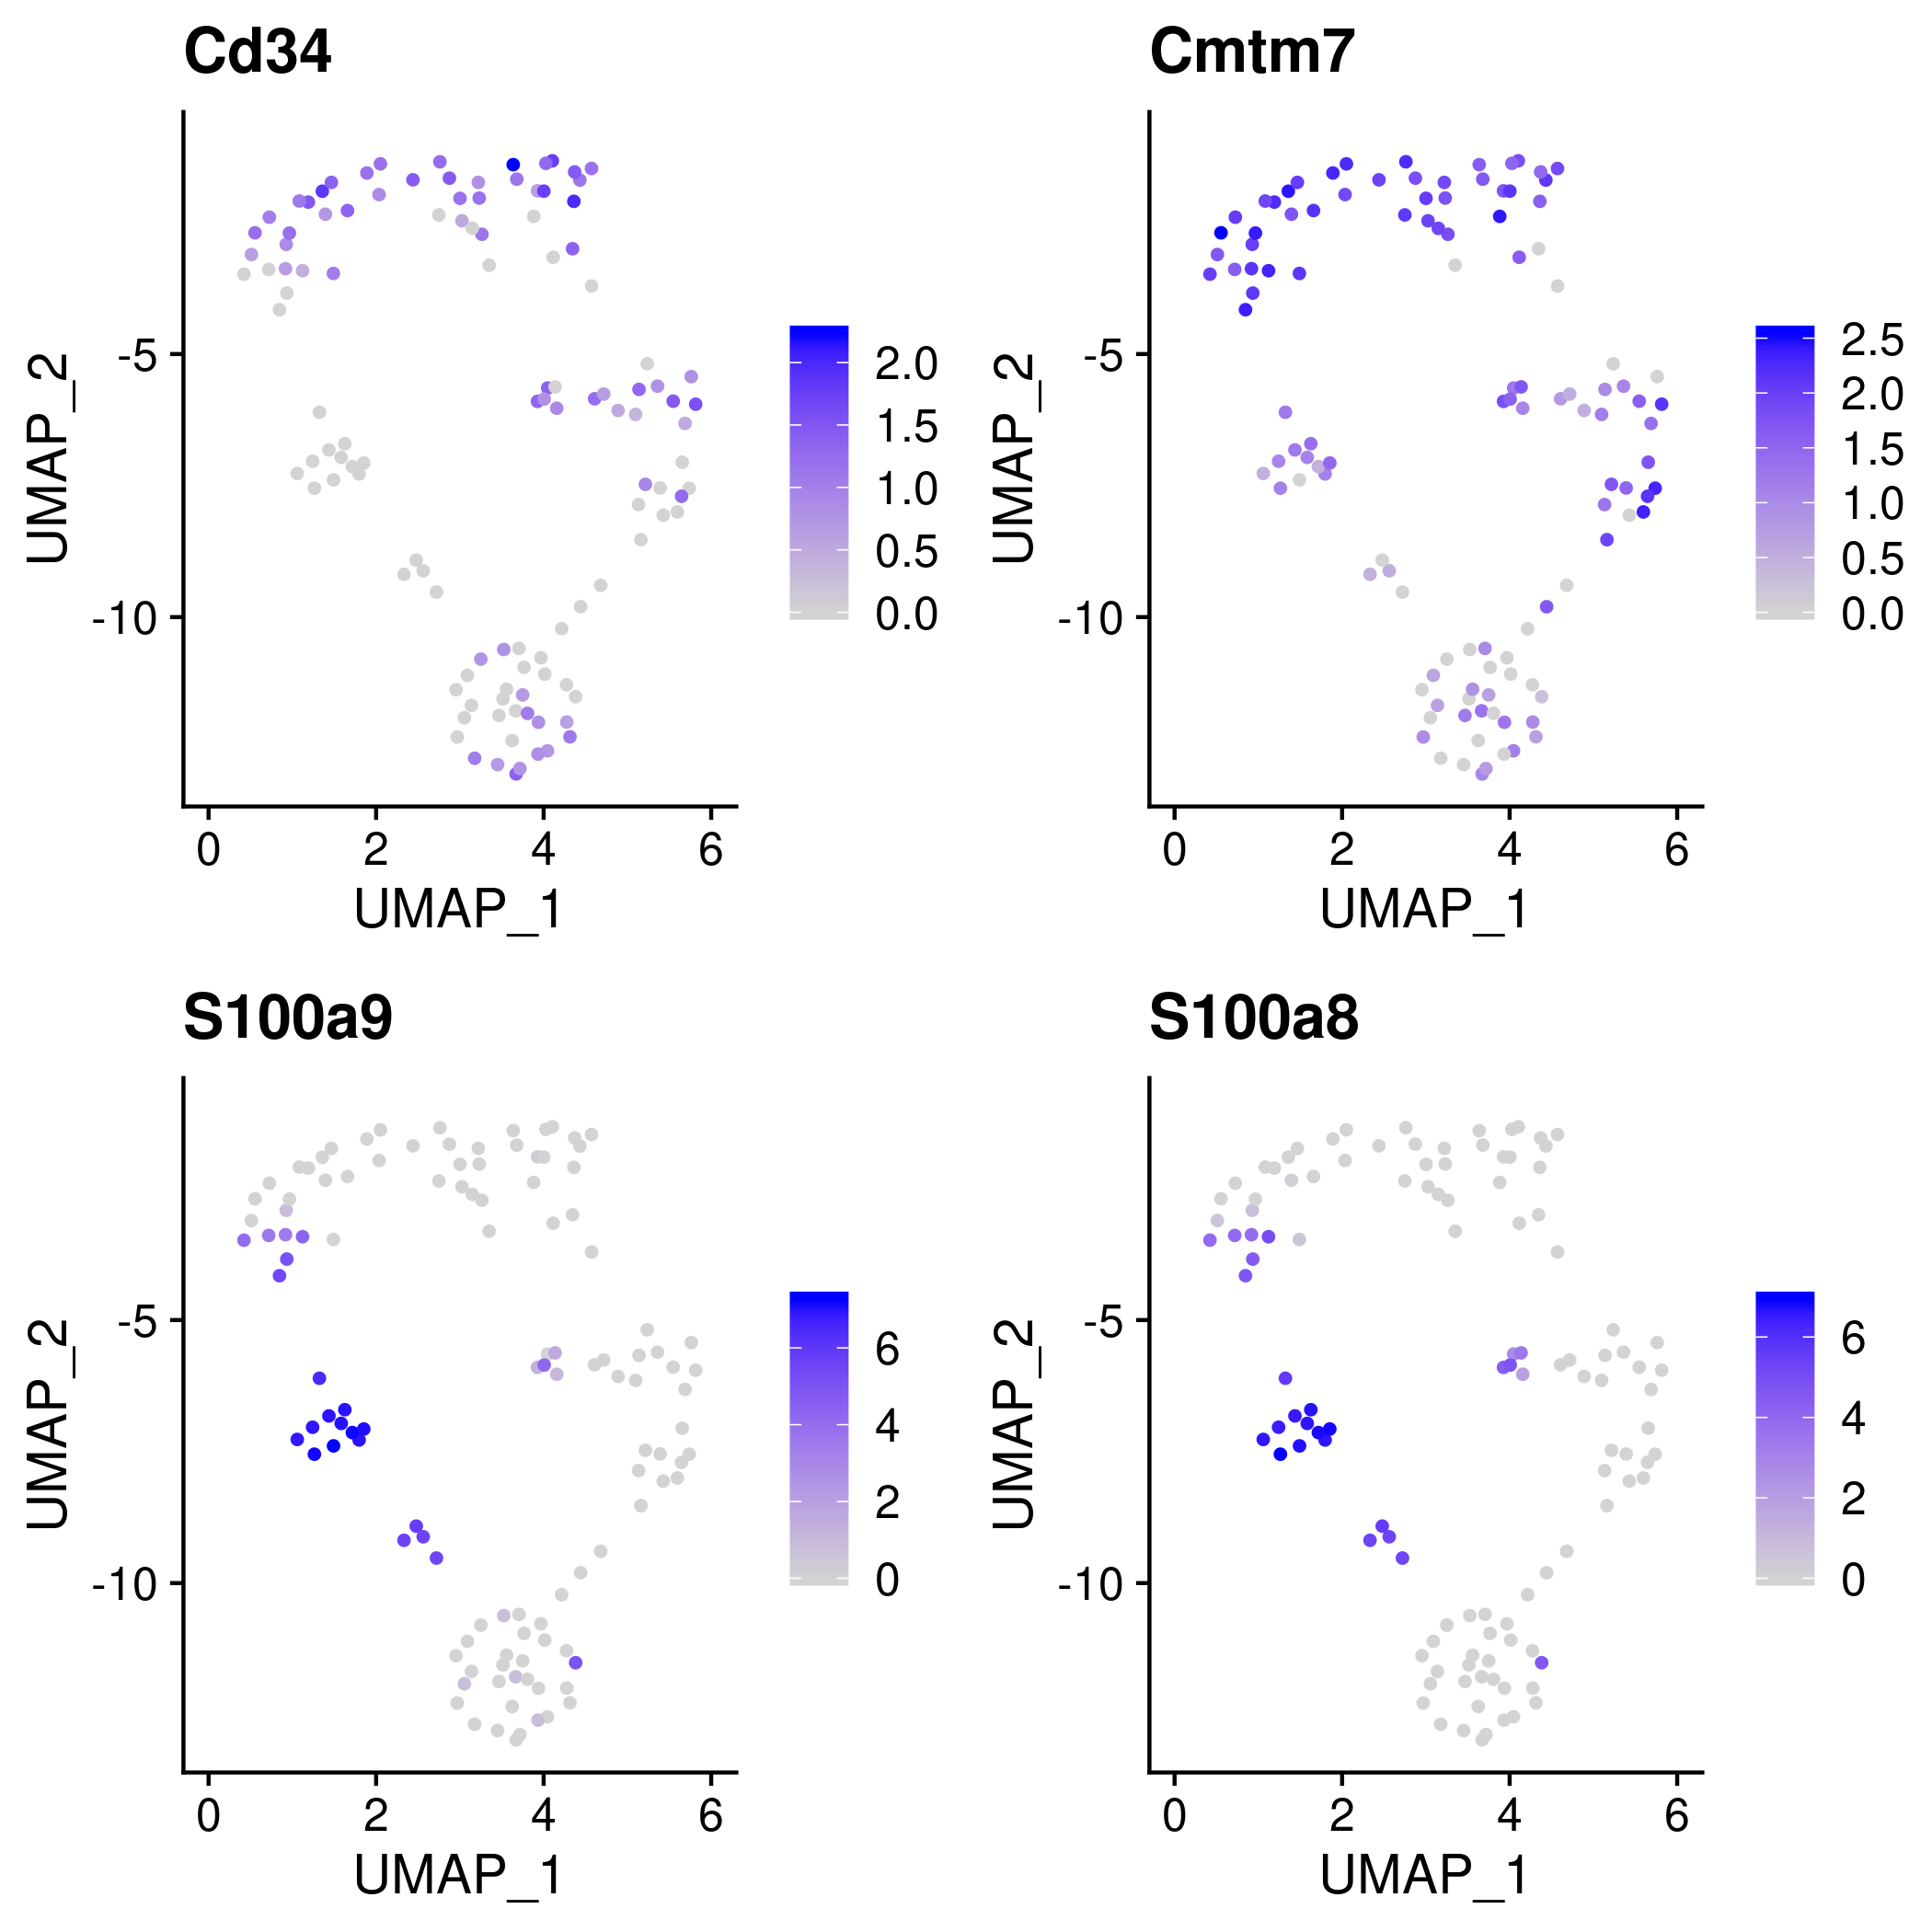
\includegraphics[width=0.6\linewidth]{image/f10.png}
    \caption{Stem and Neutrophil Markers in C10 \label{f10}}
\end{figure}
\begin{figure}[htbp]
    \centering
    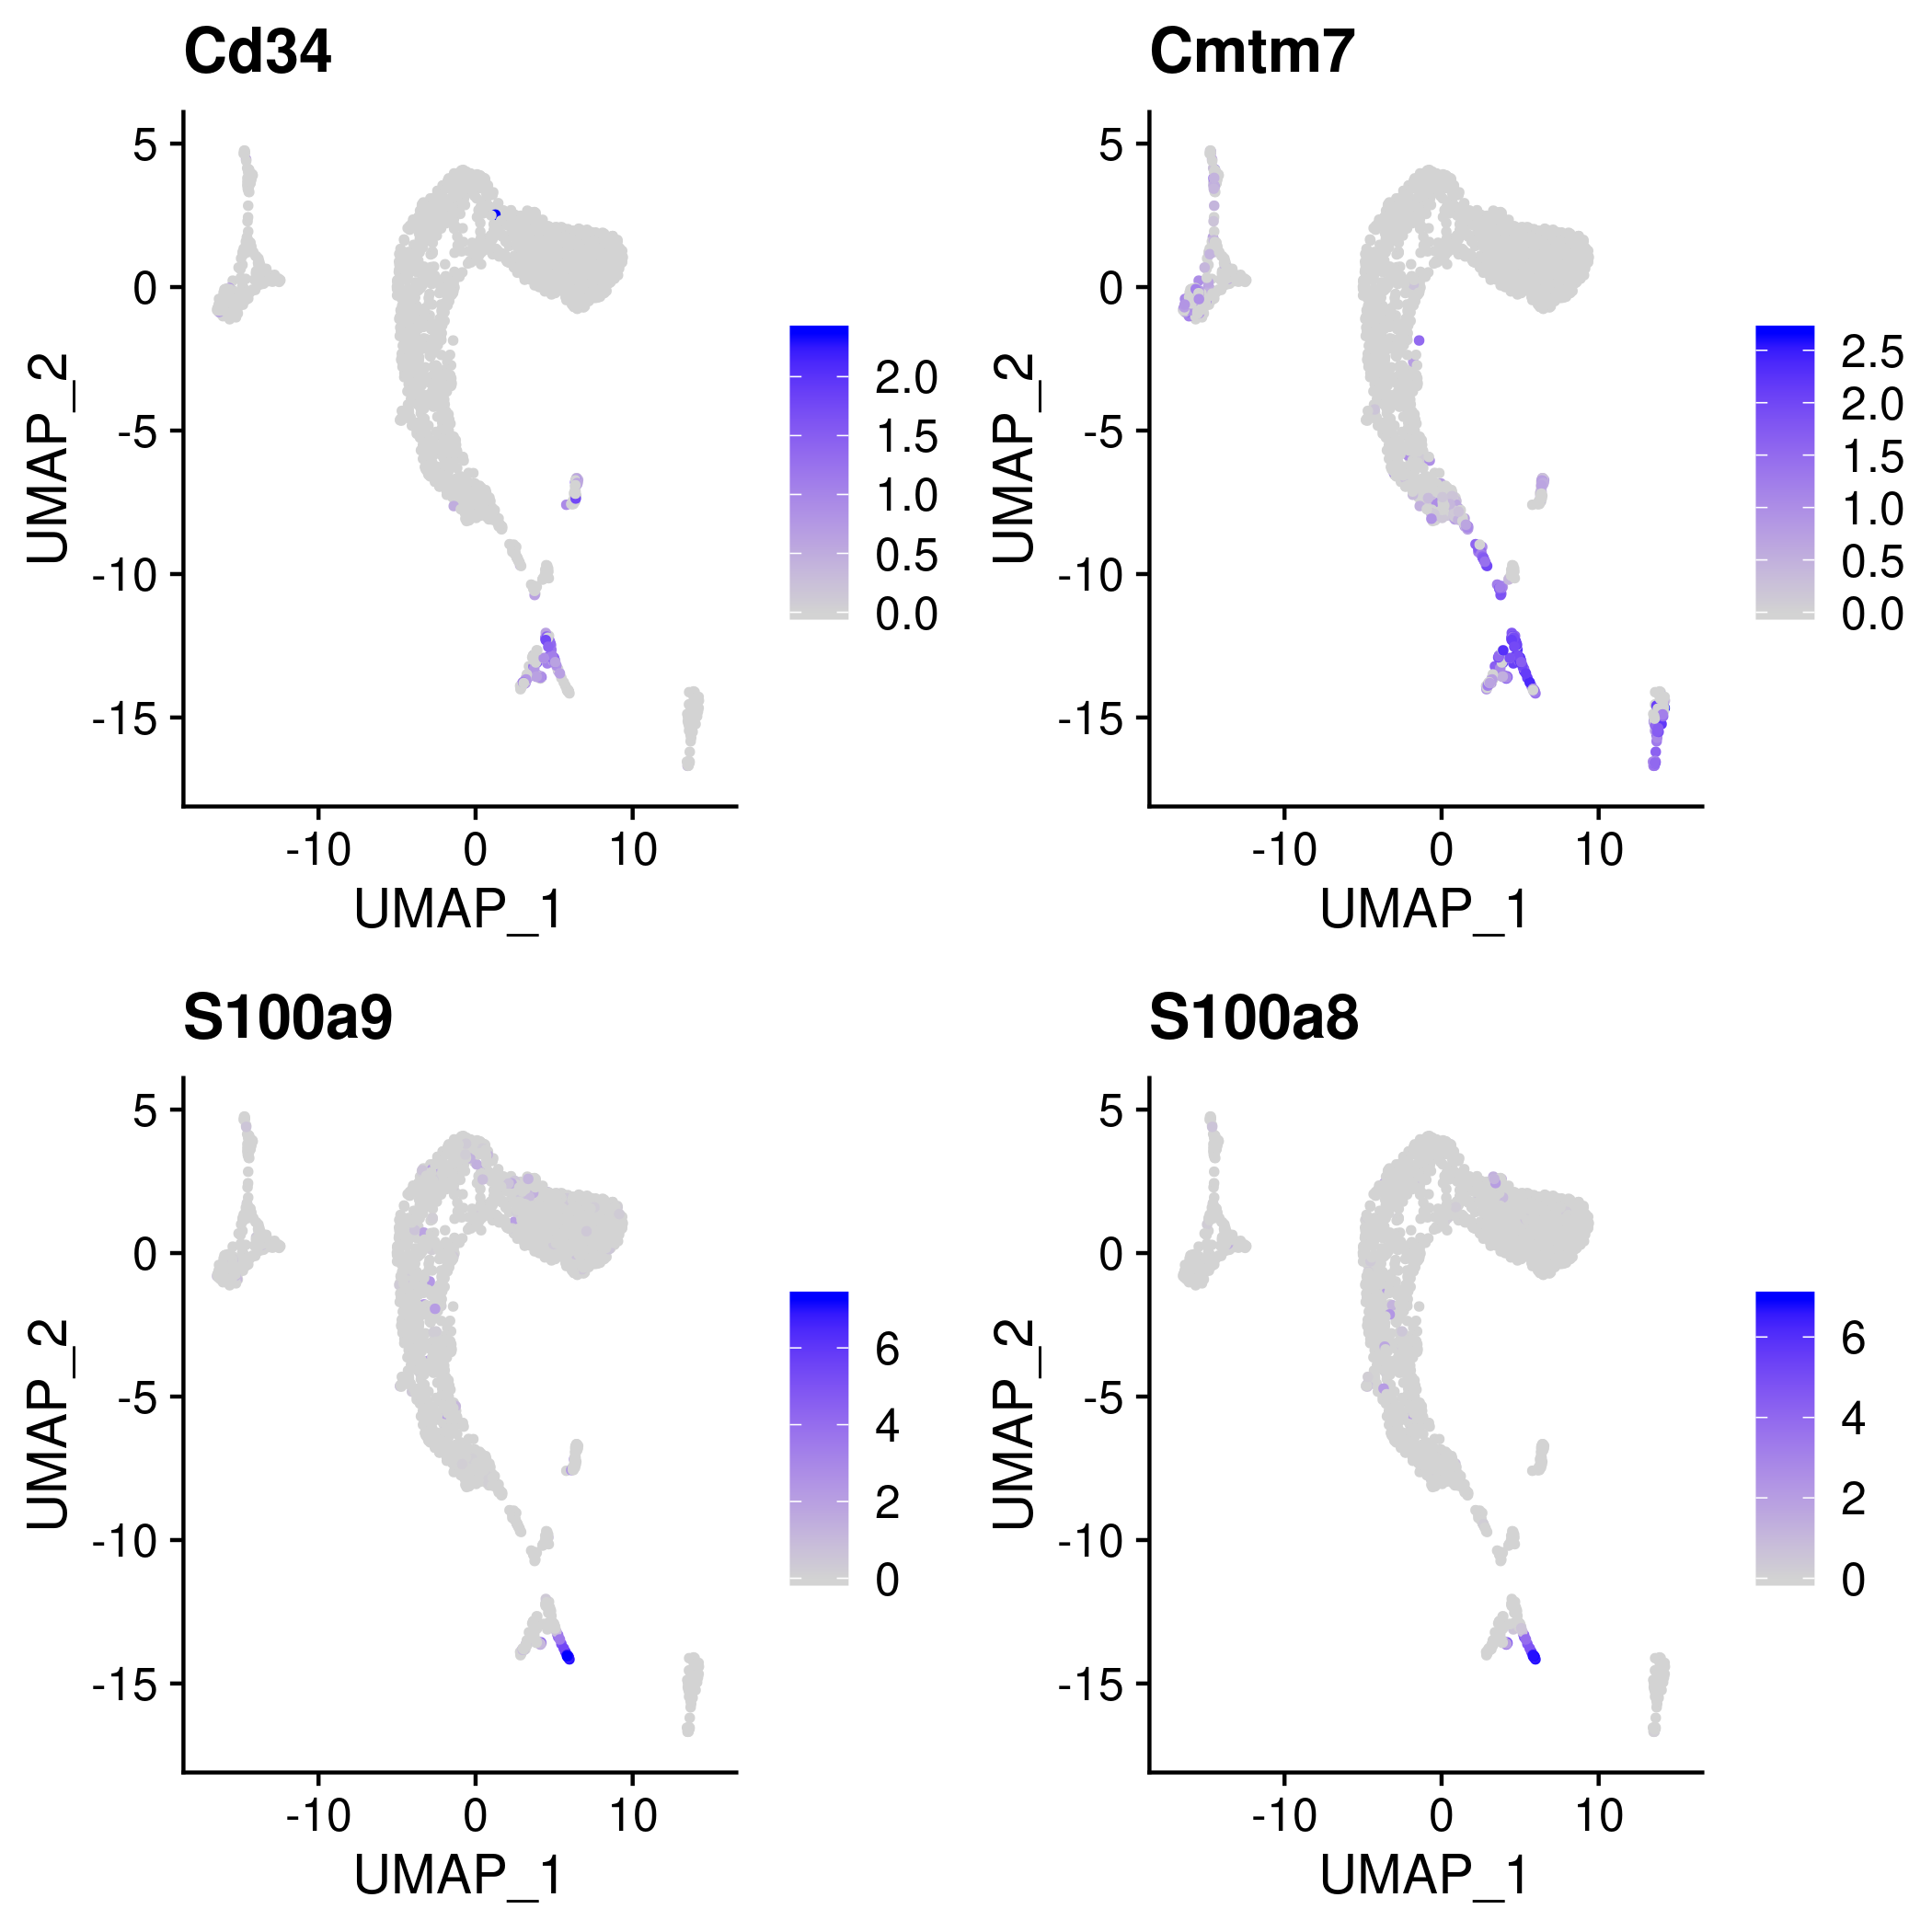
\includegraphics[width=0.6\textwidth]{image/f10t.png}
    \caption{Stem and Neutrophil Markers in Whole Data \label{f10t}}
\end{figure}

\paragraph{Cluster 11} C11 is divided into 2 parts as expected (\figref{d11}), one of which is annotated as endothelial cell and the other is annotated as mesenchymal cell, due to the endothelial marker \emph{Lyve1, Kdr}\citep{gordillo_orchestrating_2015} in subcluster 0, and the mesenchymal marker \emph{Pdgfra, Col1a2}\citep{han_mapping_2018} in subcluster 1 (\figref{f11}, \figref{f11t}). The \lstinline{.rds} file is saved at \lstinline{/p200/liujiang_group/yinyao/Dataset/Seurat/liver11.rds}

\begin{figure}[htbp]
    \centering
    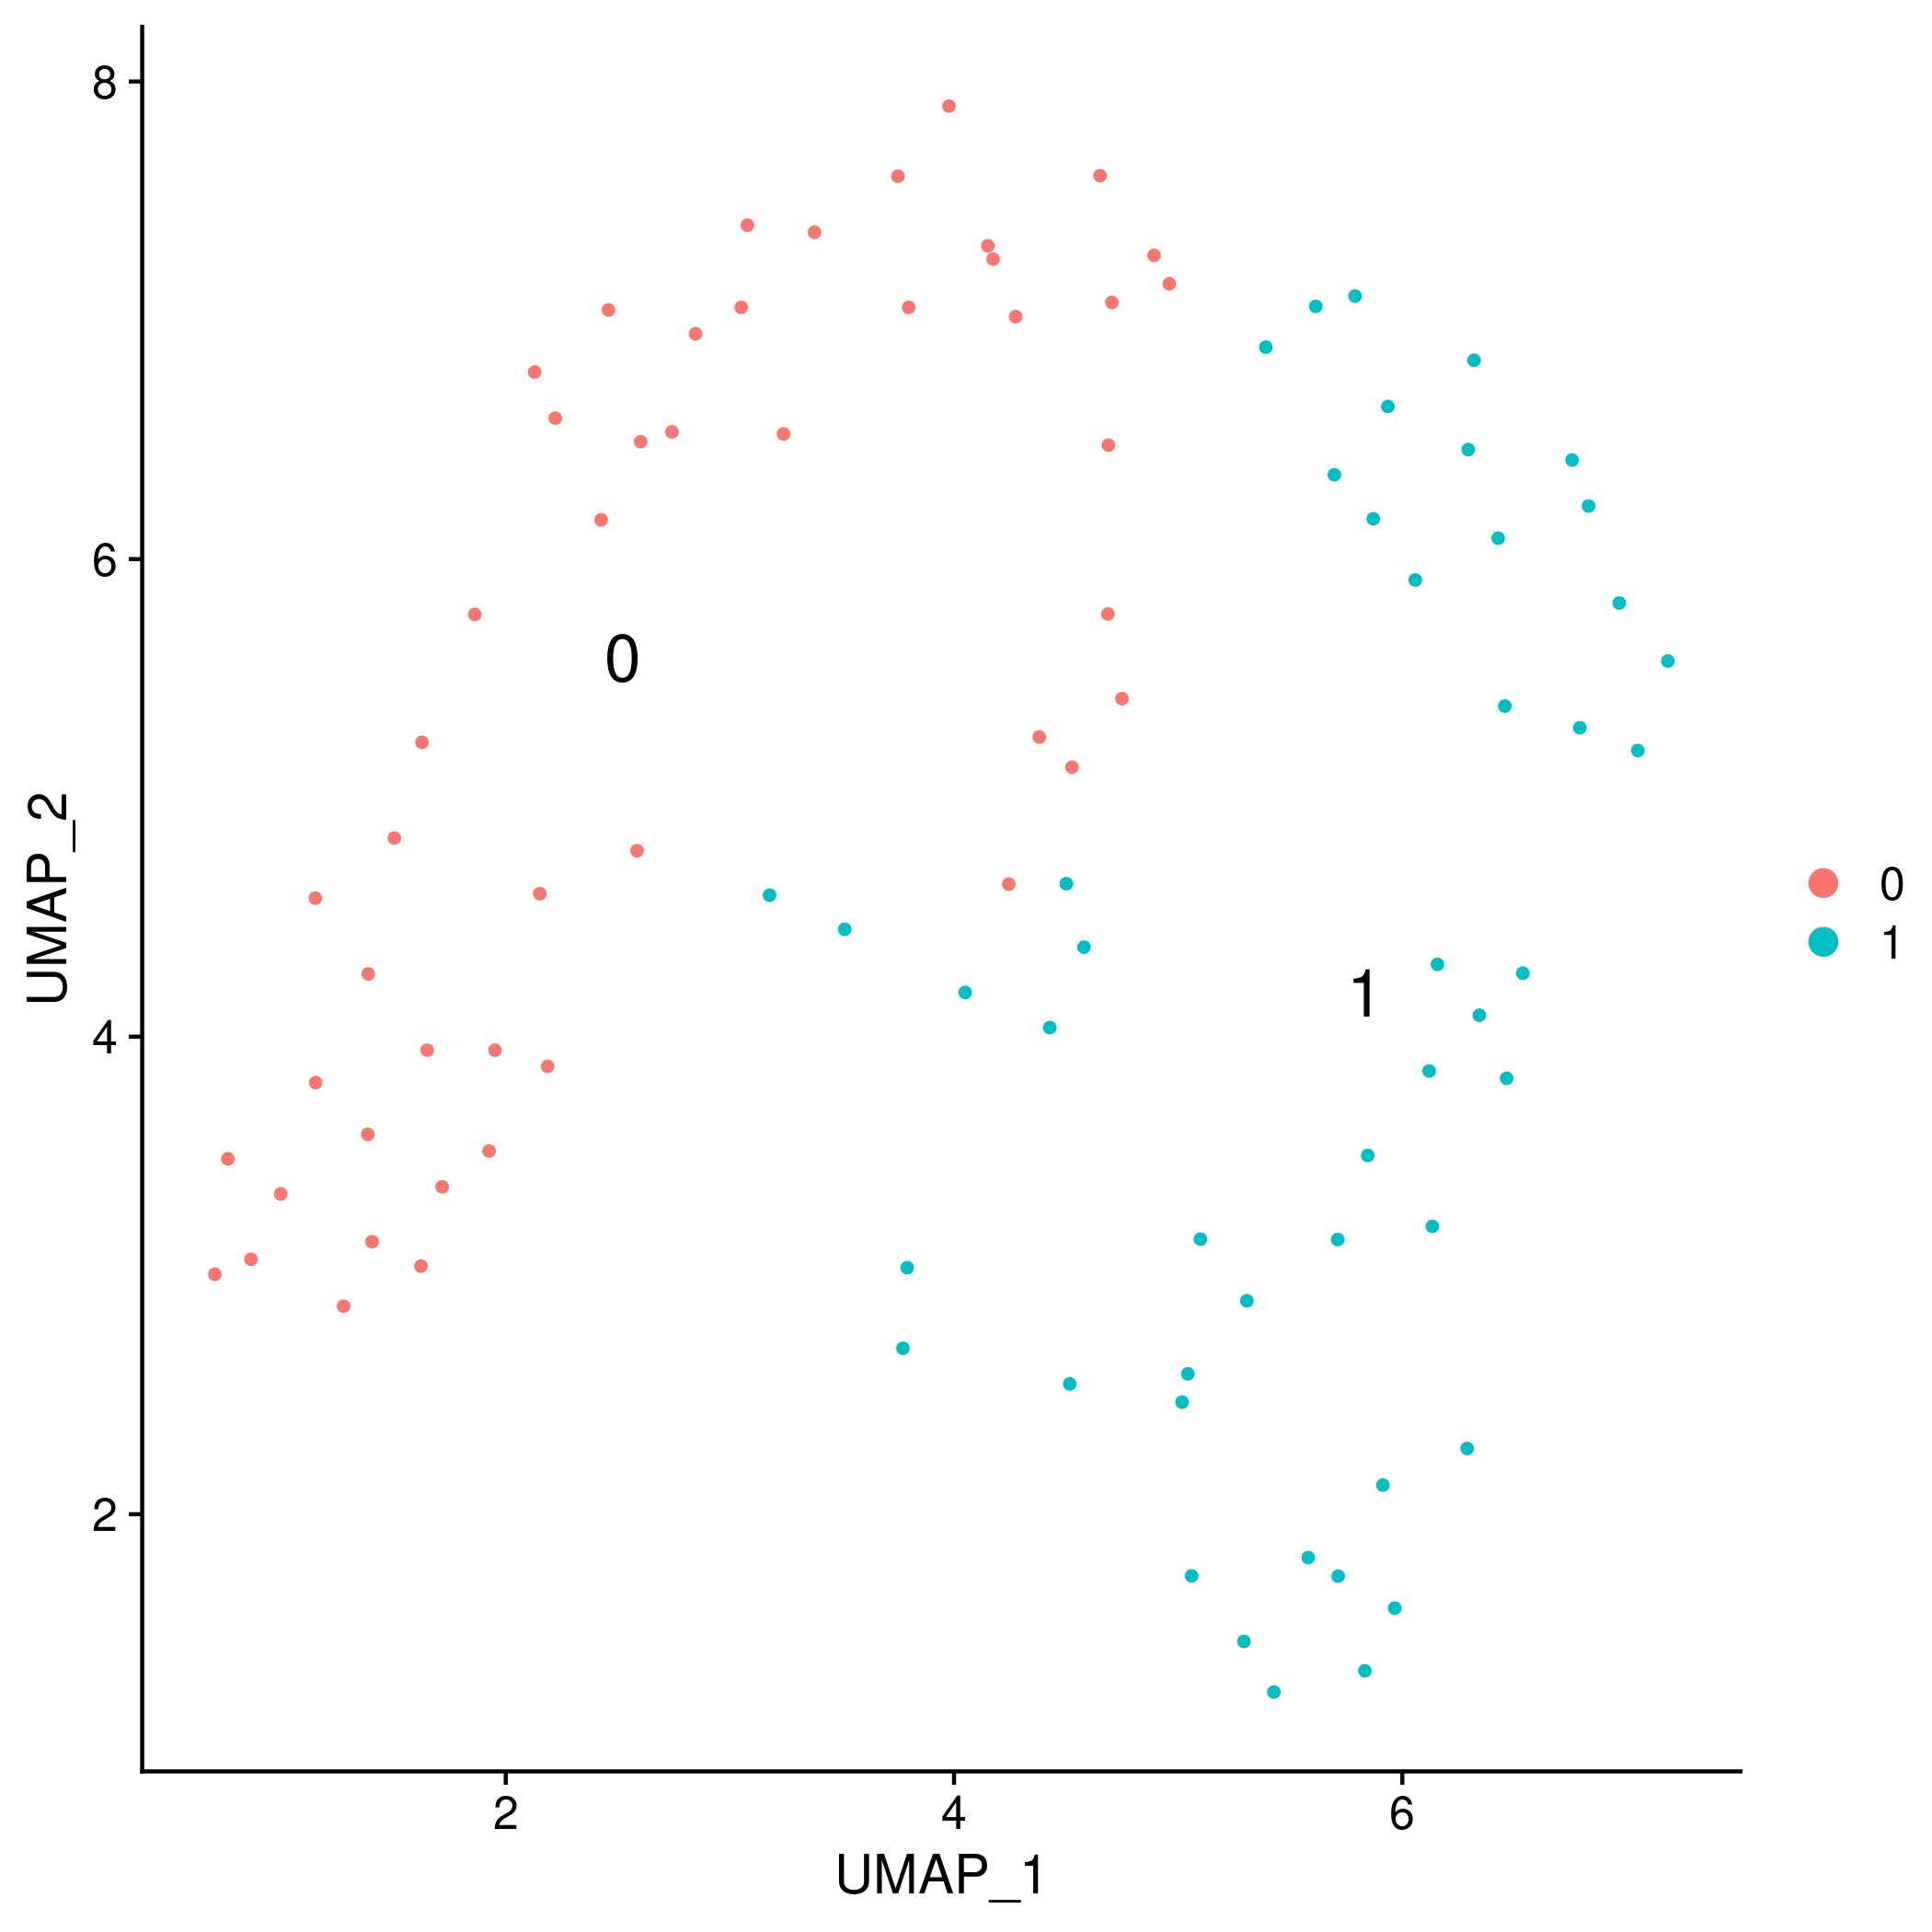
\includegraphics[width=0.6\linewidth]{image/d11.png}
    \caption{Subclusters of C11 \label{d11}}
\end{figure}
\begin{figure}[htbp]
    \centering
    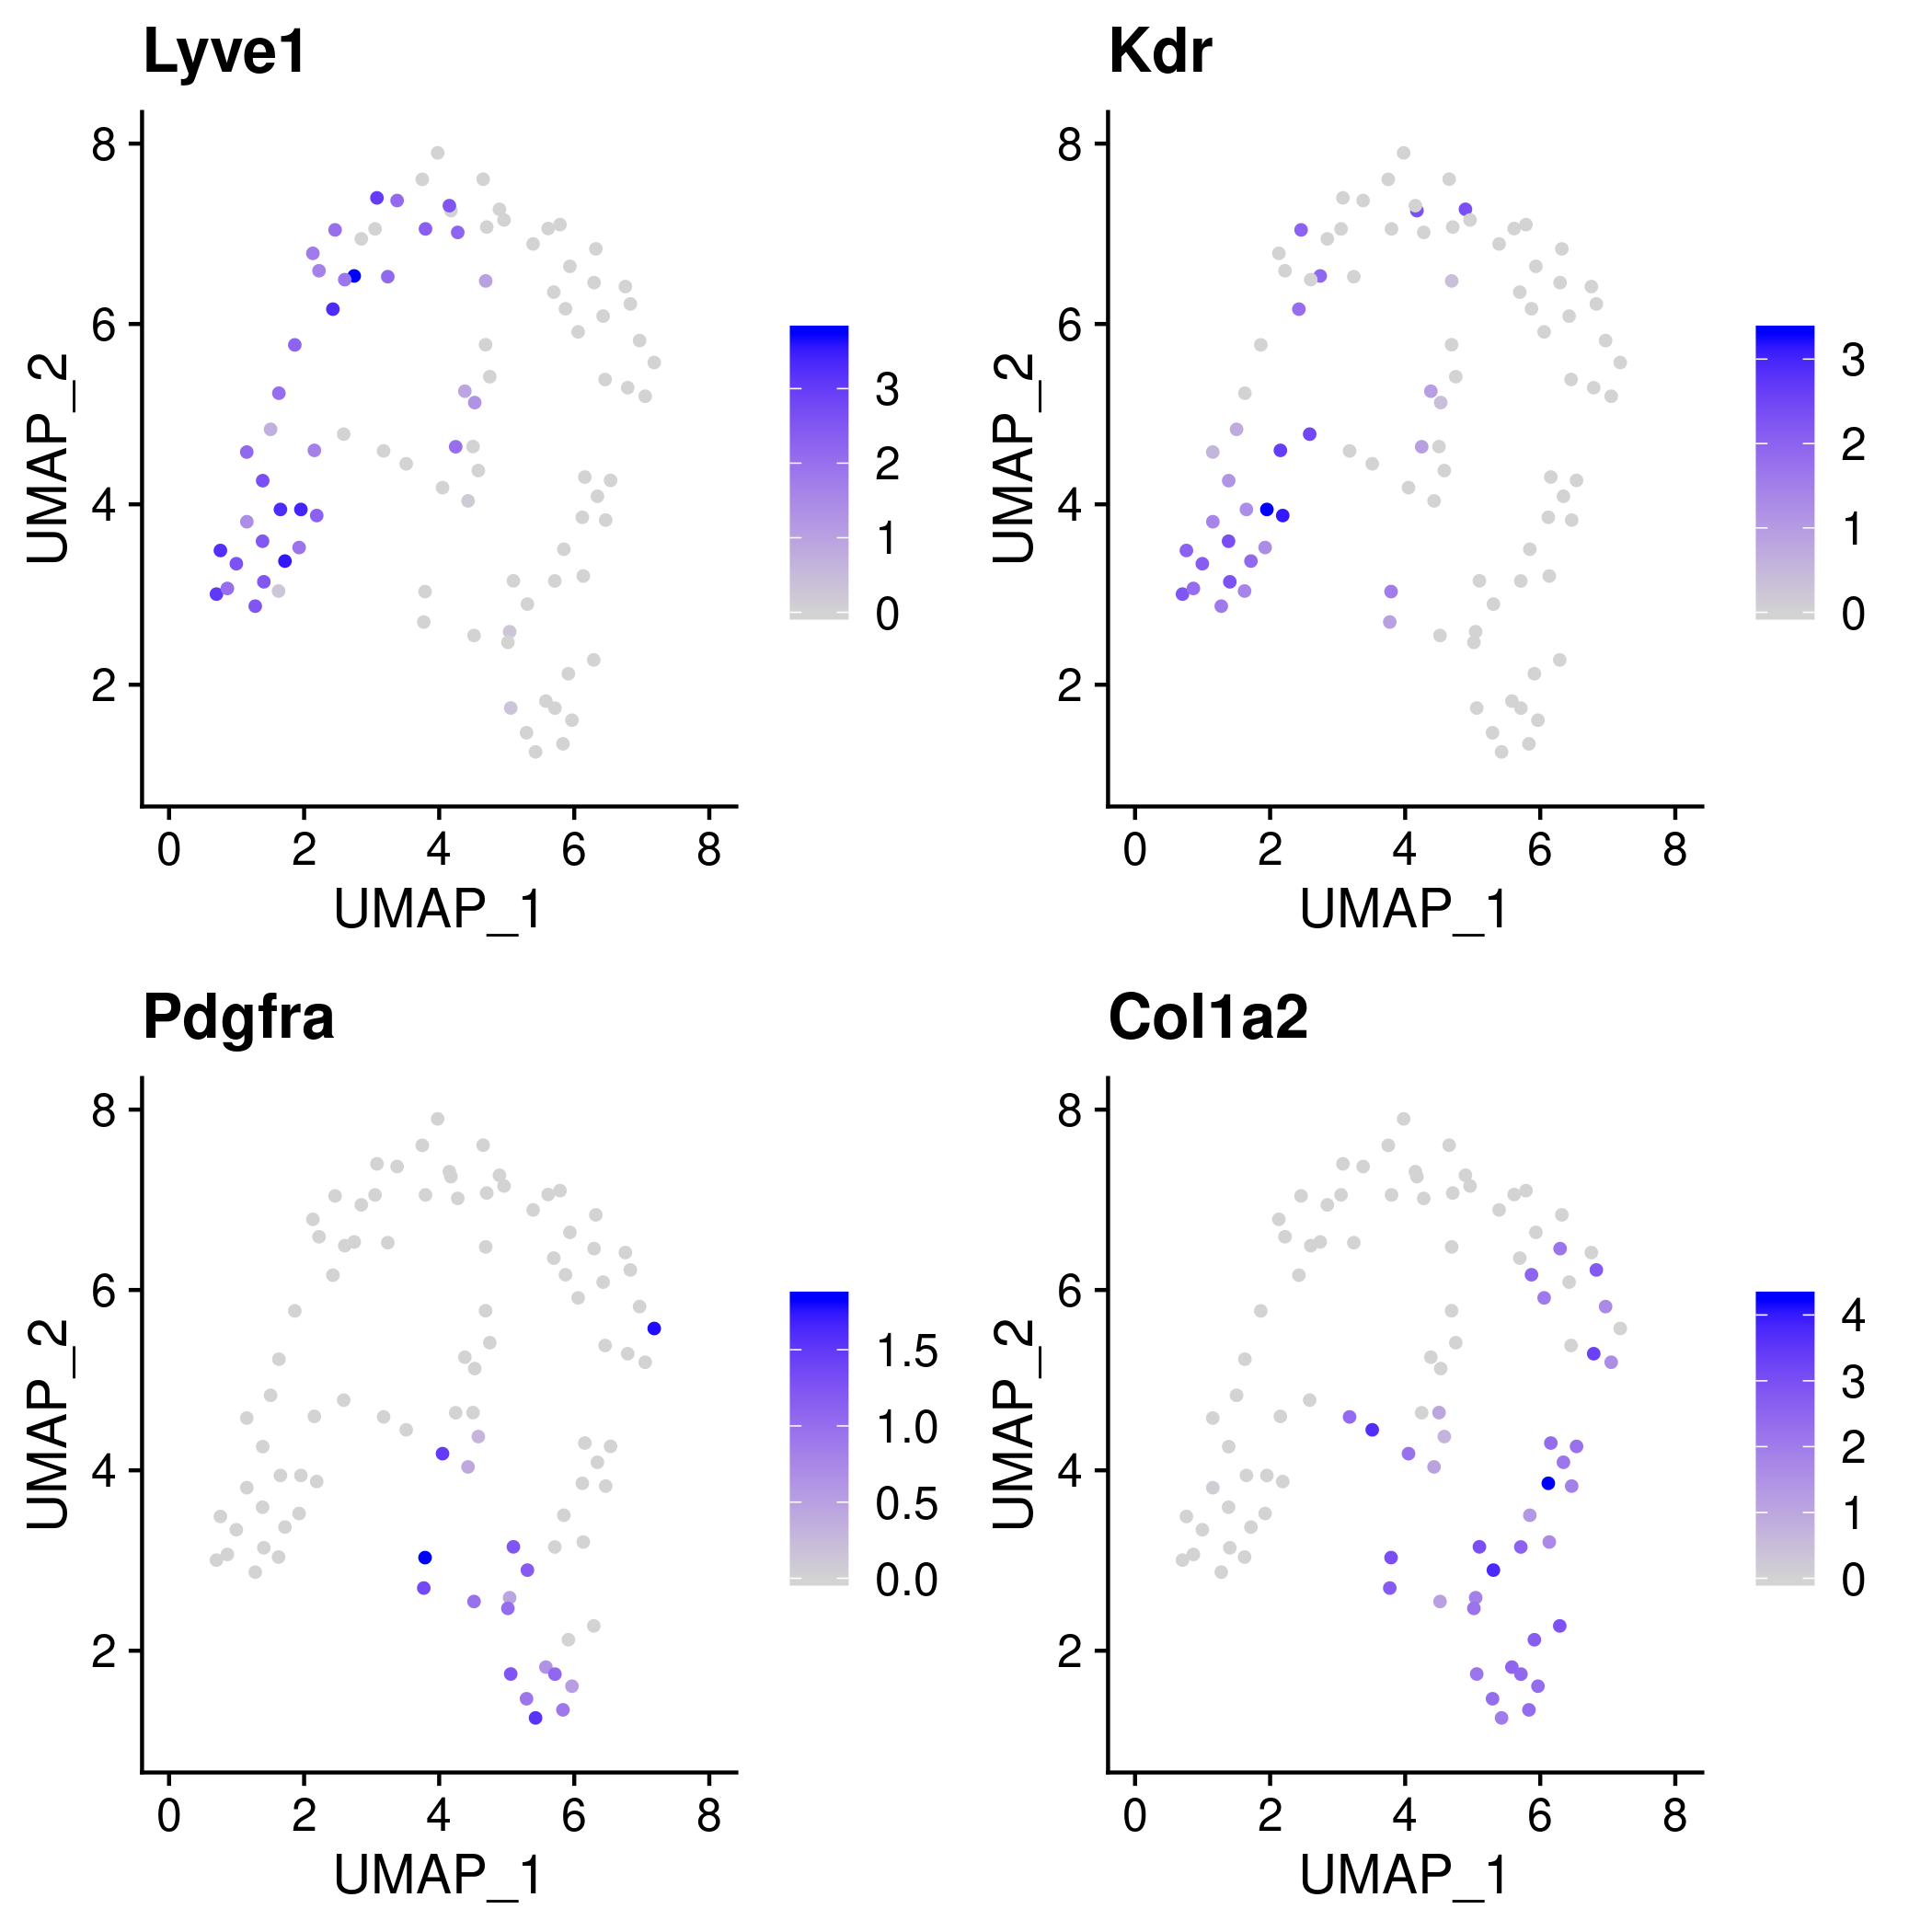
\includegraphics[width=0.6\linewidth]{image/f11.png}
    \caption{Endothelial and Mesenchymal Markers in C11 \label{f11}}
\end{figure}
\begin{figure}[htbp]
    \centering
    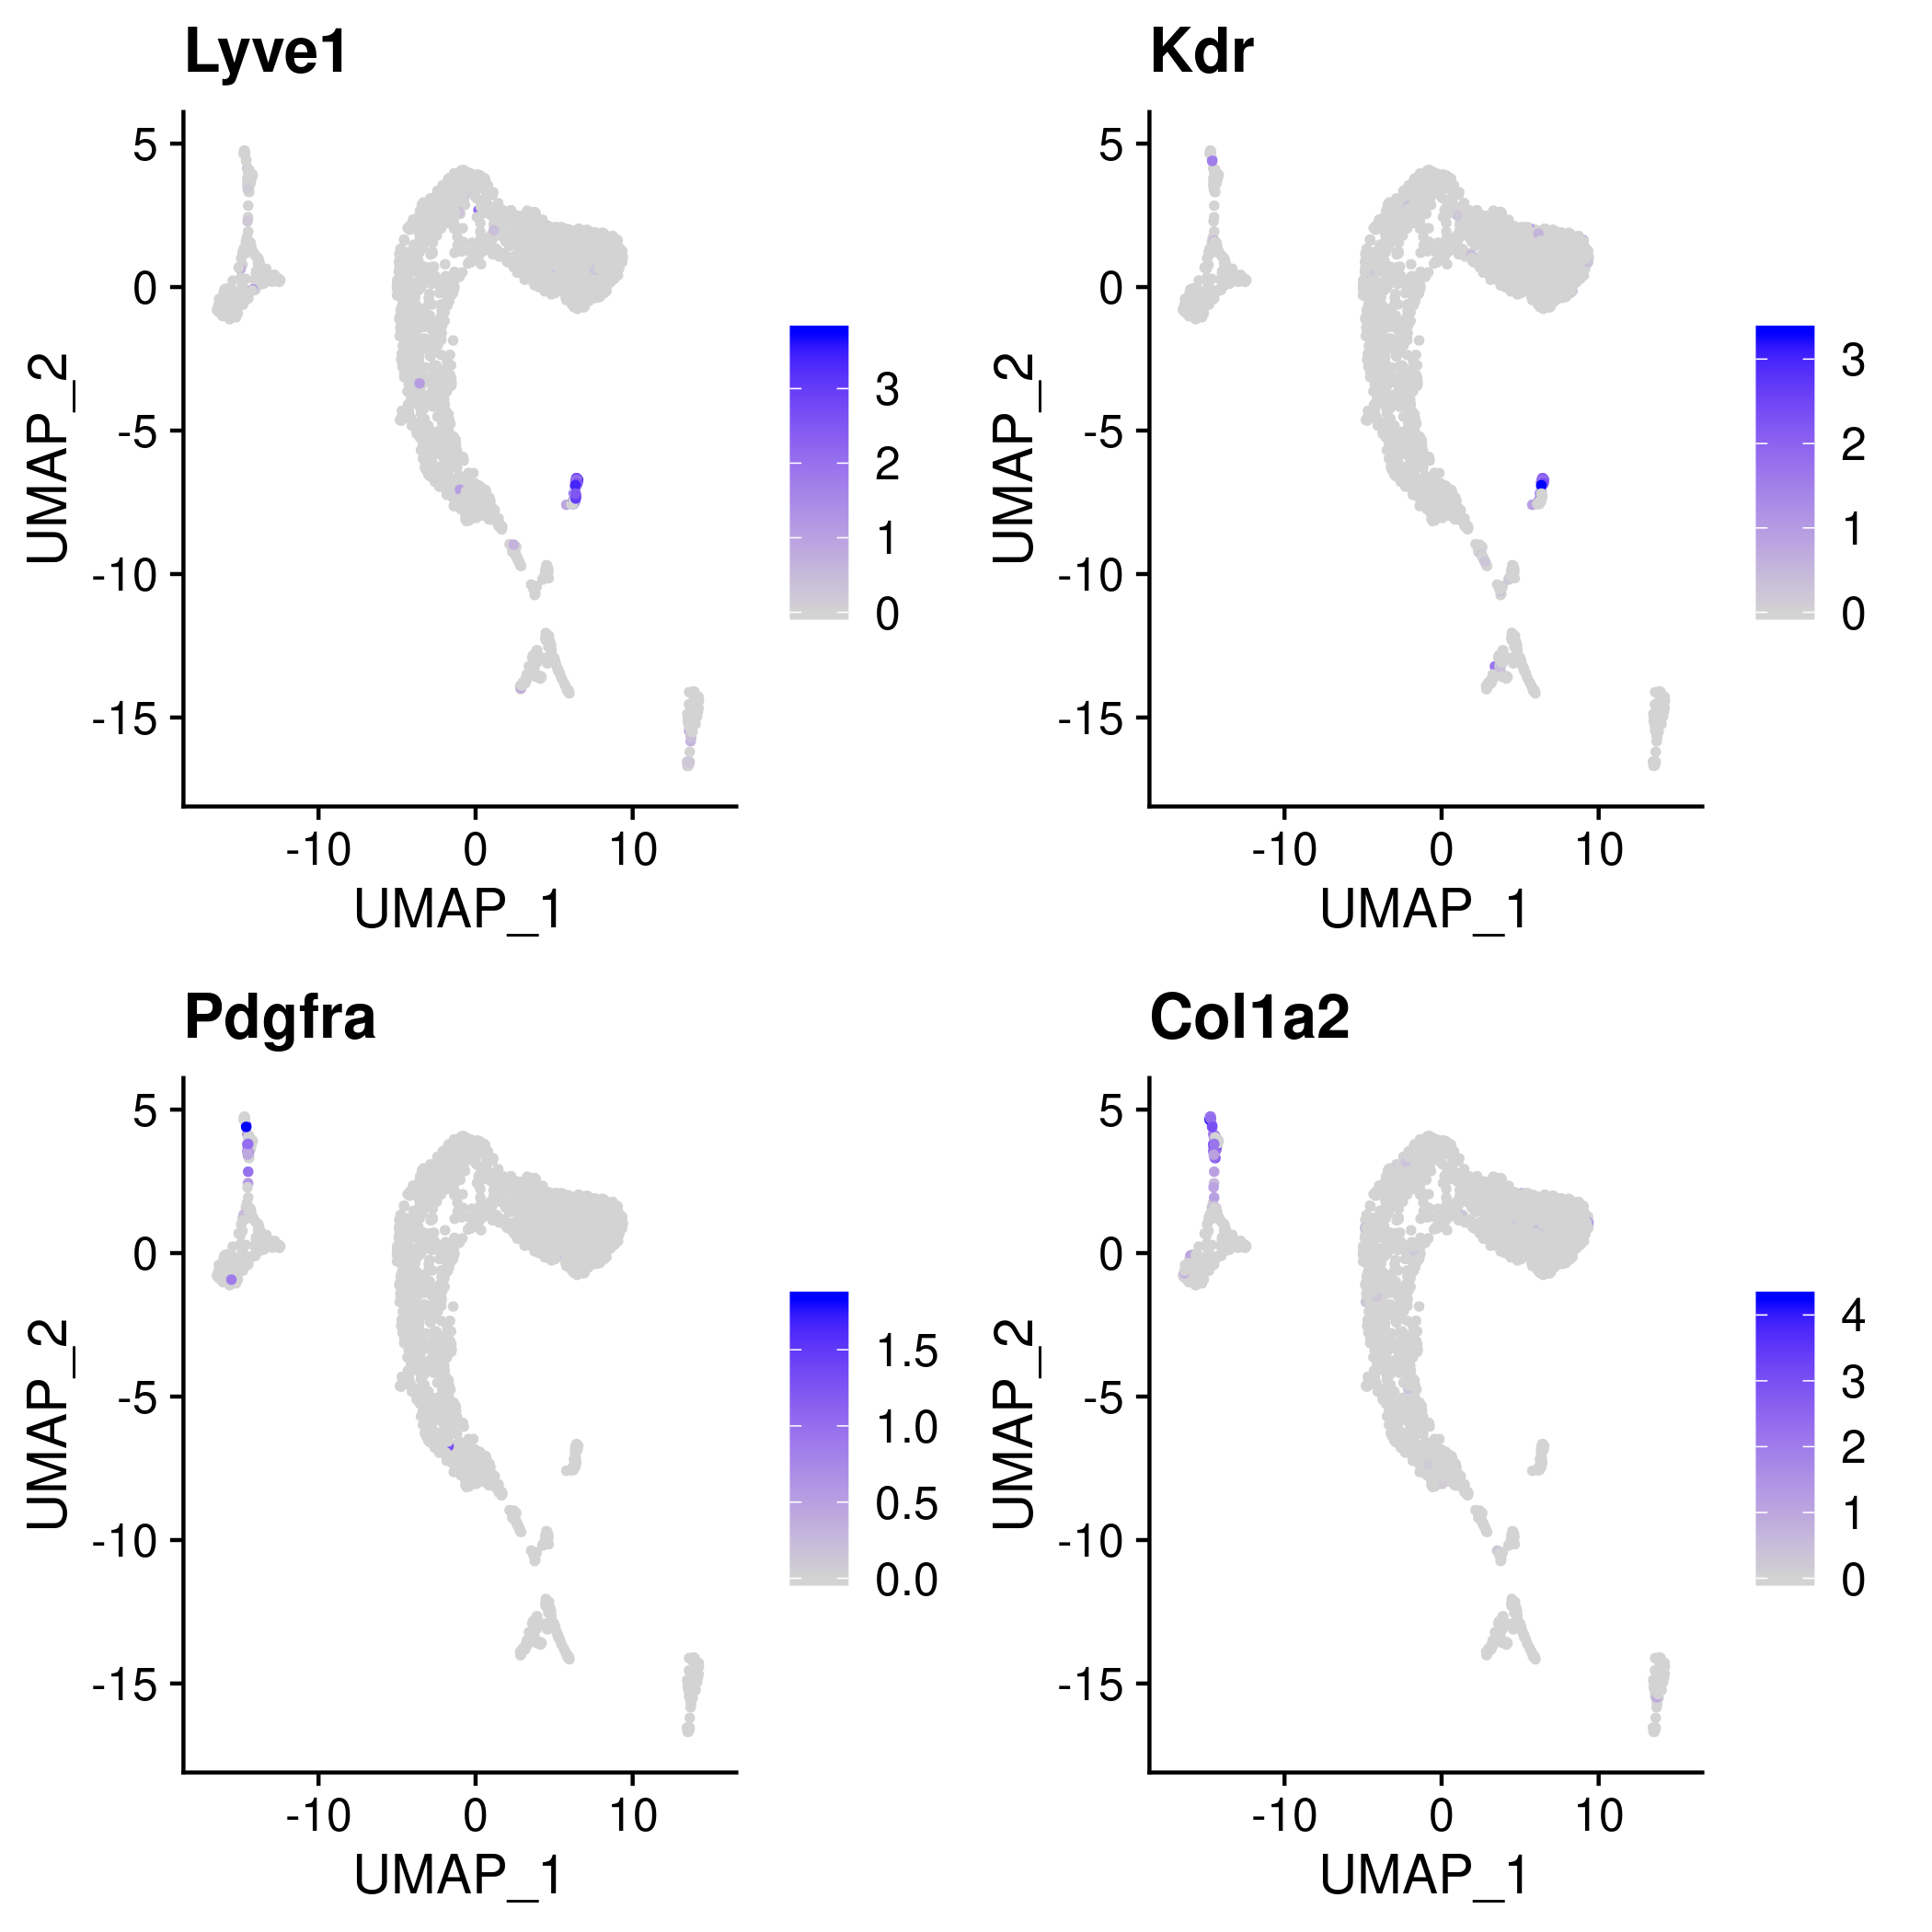
\includegraphics[width=0.6\textwidth]{image/f11t.png}
    \caption{Endothelial and Mesenchymal Markers in Whole Data \label{f11t}}
\end{figure}

\subsection{Final Annotation}

Except cell type of C3 and subcluster 1 of C10 is not defined yet, their labels maintain 3 and 10 in \figref{dt}. And the final \lstinline{.rds} file is available at \lstinline{/p200/liujiang_group/yinyao/Dataset/Seurat/liver_labeled.rds}.

\begin{figure}[htbp]
    \centering
    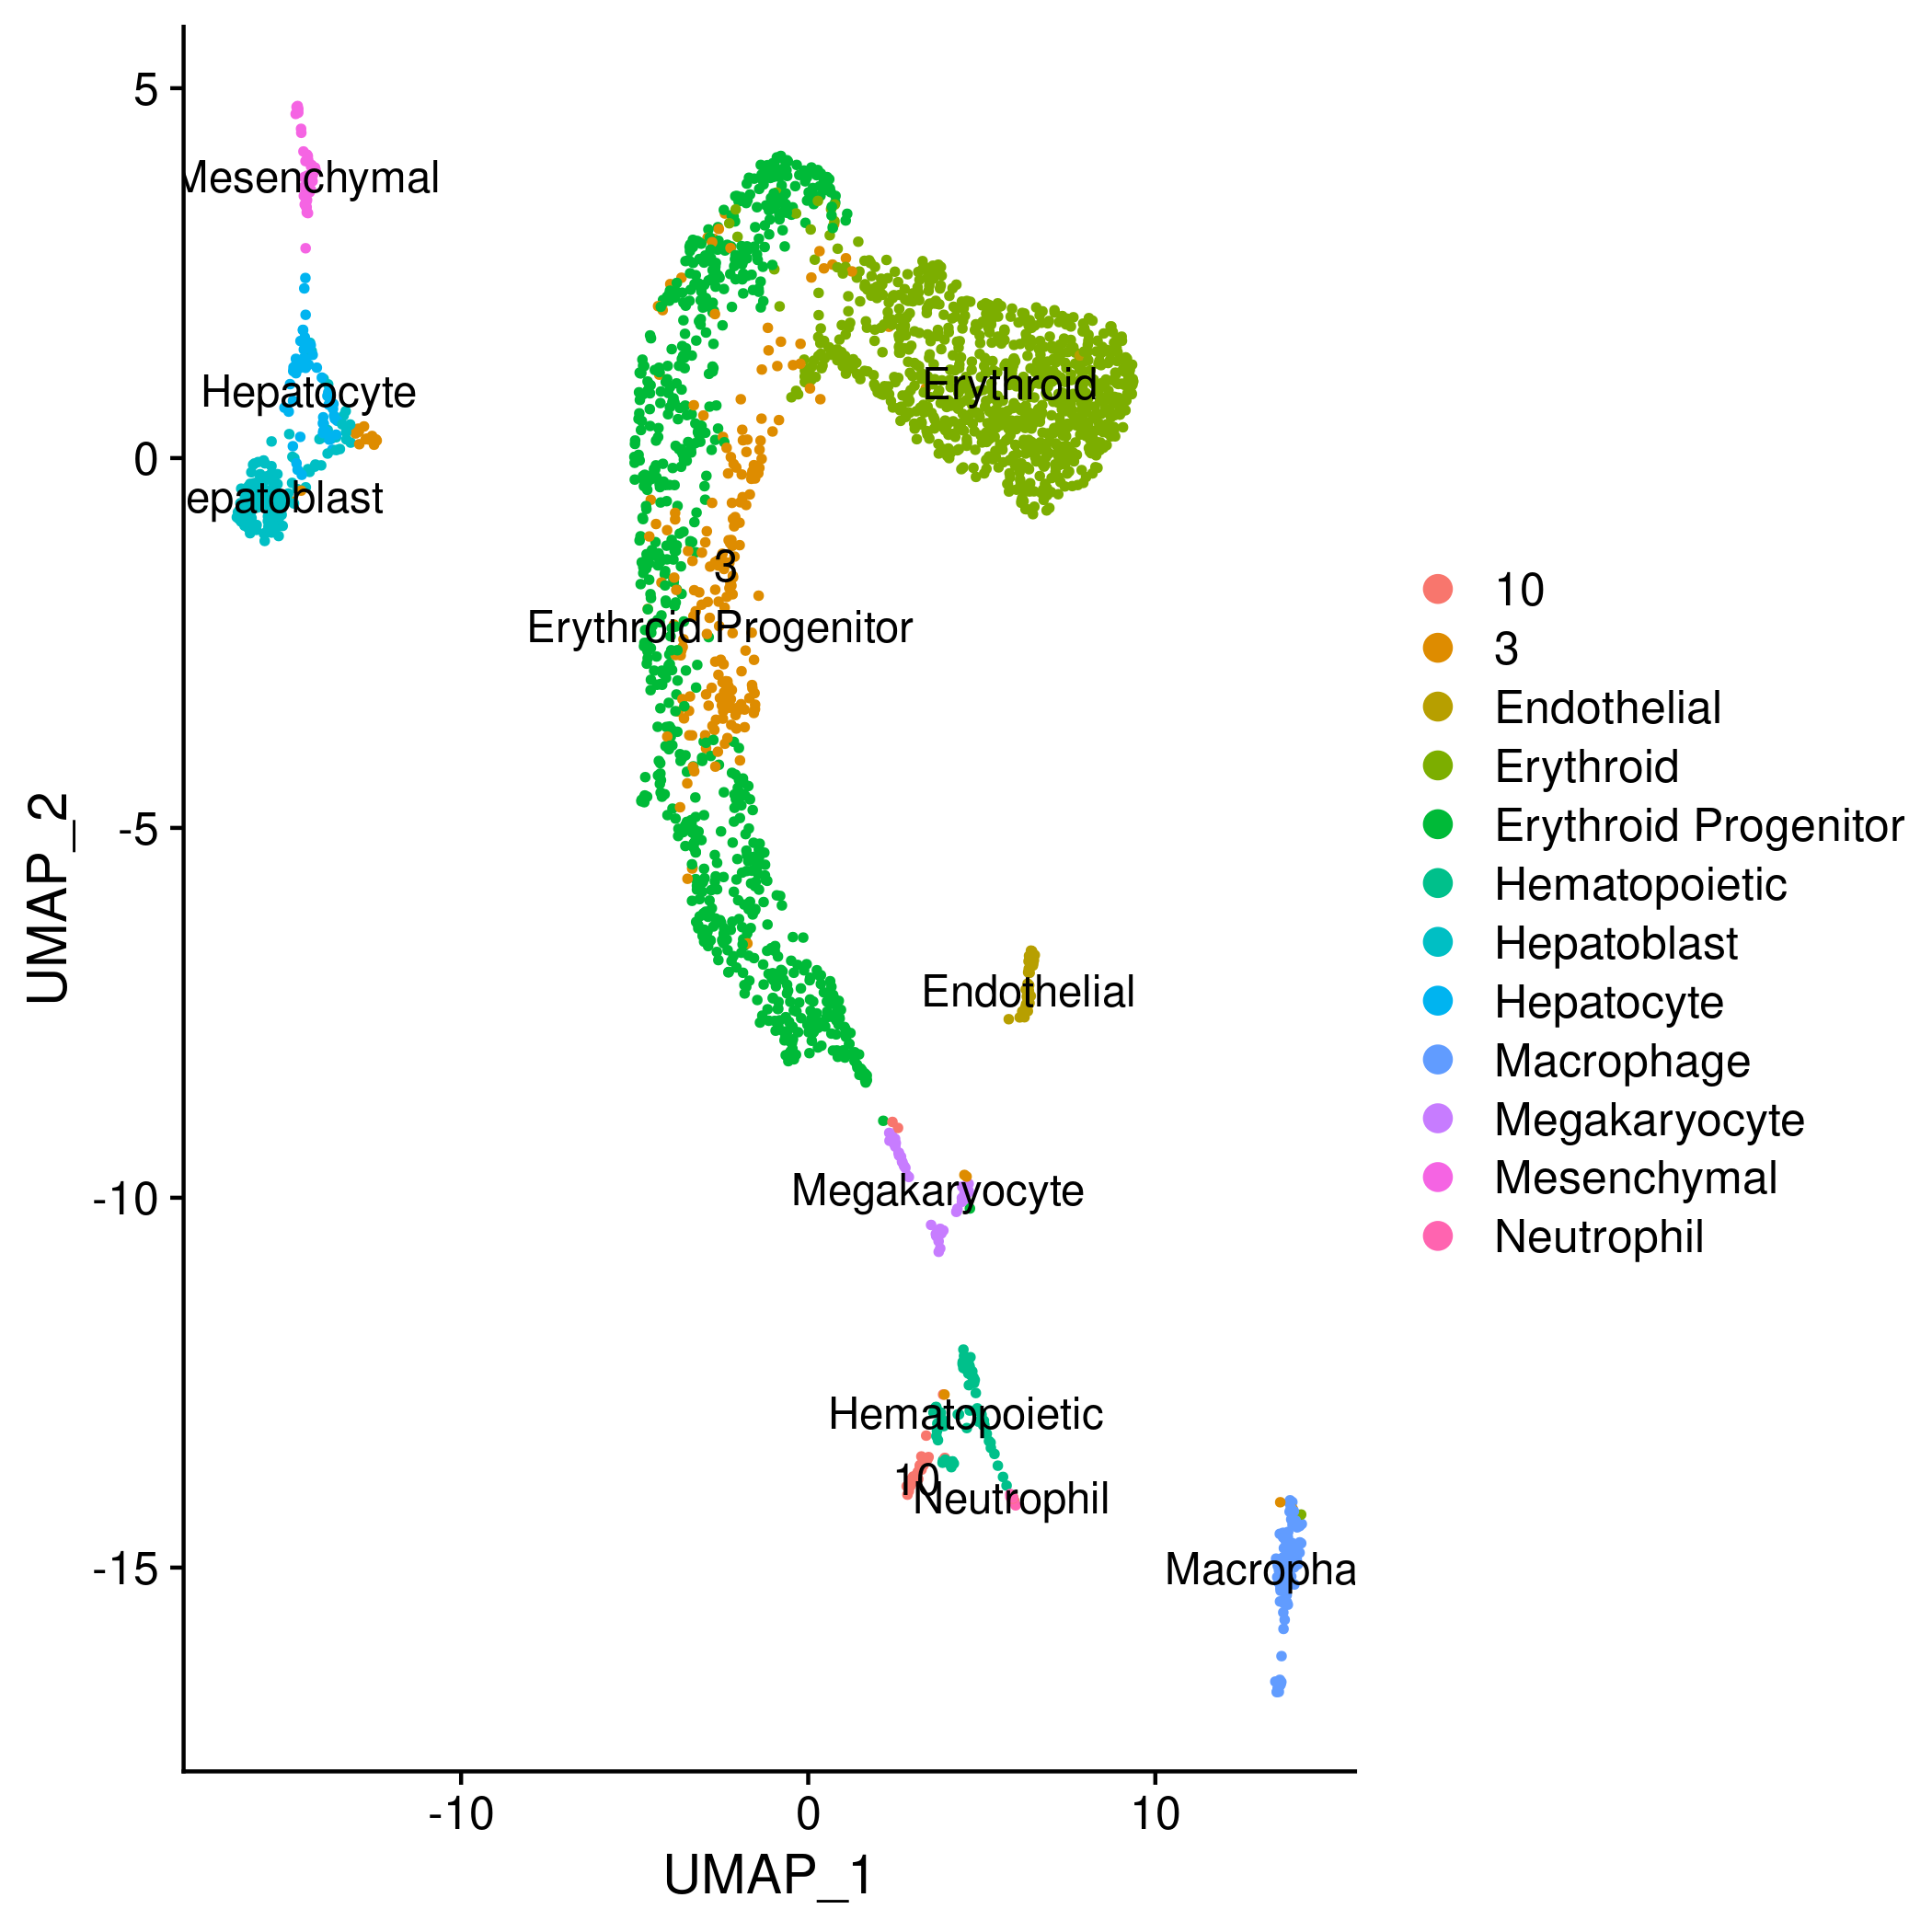
\includegraphics[width=0.6\textwidth]{image/dt.png}
    \caption{Final Annotation\label{dt}}
\end{figure}

\bibliography{LiverDevelopment}

\end{document}
